%% 
%% Copyright 2007, 2008, 2009 Elsevier Ltd
%% 
%% This file is part of the 'Elsarticle Bundle'.
%% ---------------------------------------------
%% 
%% It may be distributed under the conditions of the LaTeX Project Public
%% License, either version 1.2 of this license or (at your option) any
%% later version.  The latest version of this license is in
%%    http://www.latex-project.org/lppl.txt
%% and version 1.2 or later is part of all distributions of LaTeX
%% version 1999/12/01 or later.
%% 
%% The list of all files belonging to the 'Elsarticle Bundle' is
%% given in the file `manifest.txt'.
%% 
%% Template article for Elsevier's document class `elsarticle'
%% with harvard style bibliographic references
%% SP 2008/03/01

\documentclass[preprint,12pt,authoryear]{elsarticle}

%% Use the option review to obtain double line spacing
%% \documentclass[authoryear,preprint,review,12pt]{elsarticle}

%% Use the options 1p,twocolumn; 3p; 3p,twocolumn; 5p; or 5p,twocolumn
%% for a journal layout:
%% \documentclass[final,1p,times,authoryear]{elsarticle}
%% \documentclass[final,1p,times,twocolumn,authoryear]{elsarticle}
%% \documentclass[final,3p,times,authoryear]{elsarticle}
%% \documentclass[final,3p,times,twocolumn,authoryear]{elsarticle}
%% \documentclass[final,5p,times,authoryear]{elsarticle}
%% \documentclass[final,5p,times,twocolumn,authoryear]{elsarticle}

%% For including figures, graphicx.sty has been loaded in
%% elsarticle.cls. If you prefer to use the old commands
%% please give \usepackage{epsfig}

%% The amssymb package provides various useful mathematical symbols
\usepackage{amssymb}
\usepackage[utf8]{inputenc}
%\usepackage[italian]{babel}
\usepackage{graphicx}
\usepackage{subfigure}
\usepackage{amsmath}
\usepackage{bm}
\usepackage{lineno}

\usepackage{graphicx}
\usepackage{xcolor}
\usepackage{colortbl}
\usepackage{fp}
\usepackage{tikz, pgfplots}
\usetikzlibrary{calc}
\usetikzlibrary{patterns}
\usetikzlibrary{intersections}
\usetikzlibrary{arrows}
\tikzset{>=latex}

% Color definition
\definecolor{green2}{RGB}{154, 205, 50}
\definecolor{green3}{RGB}{141, 182, 0}
\definecolor{blue2}{RGB}{0, 102, 255}
\definecolor{lightgreen}{RGB}{178,255,102}


%% The amsthm package provides extended theorem environments
%% \usepackage{amsthm}

%% The lineno packages adds line numbers. Start line numbering with
%% \begin{linenumbers}, end it with \end{linenumbers}. Or switch it on
%% for the whole article with \linenumbers.
%% \usepackage{lineno}

\journal{Comput. Methods Appl. Mech. Eng}

\begin{document}

\begin{frontmatter}

%% Title, authors and addresses

%% use the tnoteref command within \title for footnotes;

%% use the tnotetext command for theassociated footnote;
%% use the fnref command within \author or \address for footnotes;
%% use the fntext command for theassociated footnote;
%% use the corref command within \author for corresponding author footnotes;
%% use the cortext command for theassociated footnote;
%% use the ead command for the email address,
%% and the form \ead[url] for the home page:
%% \title{Title\tnoteref{label1}}
%% \tnotetext[label1]{}
%% \author{Name\corref{cor1}\fnref{label2}}
%% \ead{email address}
%% \ead[url]{home page}
%% \fntext[label2]{}
%% \cortext[cor1]{}
%% \address{Address\fnref{label3}}
%% \fntext[label3]{}

\title{Efficient Extension to Quadrilateral Element of Three 
Field Hu-Washizu 2D Elasticity Formulation Based on Biorthogonal Systems}

%% use optional labels to link authors explicitly to addresses:
%% \author[label1,label2]{}
%% \address[label1]{}
	
%% \address[label2]{}
\cortext[cor]{Corresponding author.}%: Tel. +39 0382 98.5464}

\author{B.P. Lamichhane\fnref{newcastle}}
\ead{Bishnu.Lamichhane@newcastle.edu.au}
\author{M.Pingaro\fnref{pavia}\corref{cor}}
\ead{marco.pingaro@iusspavia.it}
\author{P.Venini\fnref{pavia}}
\ead{paolo.venini@unipv.it}

%


%\address{School of Mathematical and Physical Sciences, %University of Newcastle, Callaghan, NSW 2308 \fnref{newcastle}}
%\address{Department of Civil Engineering and Architecture,
%University of Pavia, Pavia, Italy \fnref{pavia}}

\fntext[newcastle]{School of Mathematical and Physical Sciences, University of Newcastle, Callaghan, NSW 2308}
\fntext[pavia]{Department of Civil Engineering and Architecture,
University of Pavia, Pavia, Italy}

\begin{abstract}
New quadrilateral mixed finite element based on modified Hu-Washizu formulation are presented.
Hu-Washizu is a three field formulation where the unknowns are: displacement, stress and strain.
The stability and consistency of the element are obtained by adding differnt types of bubble functions at the displacement field. Different types of bubble functions are successfully investigated and analyzed. 
In order to obtain an efficient discretization scheme, we use a pair of finite element bases forming a biorthogonal system for the strain and stress. 
The biorthogonality relation allows us to statically condense out the strain and stress from the saddle-point system leading to a symmetric and positive-definite system. 
The strain and stress can be recovered in a post-processing step simply by inverting a diagonal matrix.
Numerical examples prove the efficiency and the stability of the elements in the case of incompressible limit and distorted meshes. The extension at the 3D case is straightforward.
\end{abstract}

\begin{keyword}
mixed finite elements \sep quadrilateral element \sep Hu-Washizu \sep biorthogonal systems \sep elasticity.
%% keywords here, in the form: keyword \sep keyword

%% PACS codes here, in the form: \PACS code \sep code

%% MSC codes here, in the form: \MSC code \sep code
%% or \MSC[2008] code \sep code (2000 is the default)

\end{keyword}

\end{frontmatter}

\linenumbers
\section{Introduction}\label{sec:one}
In the linear and non-linear elasticity when the Lamé constant $\lambda$ tends to infinity the standard finite element exhibit some problem of convergence may be locking phenomena.
In this context mixed formulations are used to solve this inconvenient.
One of the most popular mixed formulation adopted is the Hellinger-Raisner formulation, in that we describe the problem using with variables the stresses and the displacements.
This type of formulation requires the fulfillment of the inf-sup condition as described in \cite{boffi_book}.
For the Hellinger-Reissner formulation many elements are created such as \cite{arnold} for triangle elements and \cite{arnold_quad} for quadrilateral. 
Another type of formulation is the Hu-Washizu formulation (see \cite{hu,washizu}) that it was a three-field formulation.
This was first introduced by \cite{veubeke}.
One examples of Hu-Washizu formulation applied at linear and non-linear elasticity using quadrilaterals and hexahedra are reported in \cite{kasper_p1,kasper_p2}. 
In \cite{lamichhane_conv} are showed that the modify Hu-Washizu formulation are able to obtaining uniform convergence of the finite nelement approximation in the nearly incompressible regime in the case of quadrilateral elements.
The goal of this work is to present an extension using the quadrilateral elements of the modified three-field formulation Hu-Washizu presented in \cite{lamichhane_huwashizu}.
In accordance to \cite{lamichhane_three} we adopt the idea to create a biorthogonal system between the stresses and strains.
This assumption is essentially for the static condensation of the stresses and strains for obtain a linear system in the only unknown displacement field.
In order to ensure the stability of the element we enrich the space of displacement field with different type of bubble functions in accordance to \cite{bai,lamichhane} for the Stokes problem. 
In \cite{bai} we adopt two bubble functions to stabilize the element, while in \cite{lamichhane} use one single bubble function.  
 
The structure of the papers are the following: first of all in Section \ref{sec:two} we recall the basic equations of linear elastic problem, in Section \ref{sec:three} we briefly recall the modified Hu-Washizu formulations, Section \ref{sec:four} we develop the finite element spaces.
Finally in Section \ref{sec:five} we report some examples using the studied element and in Section \ref{sec:six} the conclusions of the work are detailed.

\section{Linear elastic continuum problem}\label{sec:two}
In this section we briefly recovery the equations governing the linear elastic problem. 
The equilibrium equation is:
\begin{equation} \label{eq:equilibrio01}
- \mbox{div}(\bm{\sigma}) = \bm{f}\:,
\end{equation}
while in small deformation is:
\begin{equation}\label{eq:congruenza01}
\bm{d} = \bm{\varepsilon}(\bm{u}) = 
\frac{1}{2}(\bm{\nabla} \: \bm{u} + \bm{\nabla} \: \bm{u}^{T}) \:.
\end{equation}
In the case of linear elasticity we have:
\begin{equation} \label{eq:legame01}
\bm{\sigma} = \lambda \: tr(\bm{\varepsilon}) \bm{I} 
+ 2\mu \: \bm{\varepsilon}
\end{equation}
where $\mu$ and $\lambda$ are the Lamé constant.
By some algebra one obtains:
\begin{equation} \label{eq:legame02}
\bm{\sigma} =
\left(
\begin{array}{cc}
\lambda (\varepsilon_{11} + \varepsilon_{22}) & 0 \\
0 & \lambda (\varepsilon_{11} + \varepsilon_{22}) 
\end{array}
\right) +2\mu
\left(
\begin{array}{cc}
\varepsilon_{11} & \varepsilon_{12} \\
\varepsilon_{12} & \varepsilon_{22}
\end{array}
\right)\:,
\end{equation}
and rearranging the equation \eqref{eq:legame02}:
\begin{equation} \label{eq:legame03}
\bm{\sigma} =
\left(
\begin{array}{ll}
(\lambda+2\mu) \varepsilon_{11} + \lambda \: \varepsilon_{22} & 2\mu \: \varepsilon_{12} \\
2\mu \: \varepsilon_{12} & (\lambda+2\mu) \: \varepsilon_{22} + \lambda \: \varepsilon_{11}  \\
\end{array}
\right)\:.
\end{equation}

\section{Briefly introduction to modify Hu-Washizu}\label{sec:three}
We define the trial variables: $\bm{\varepsilon}(\bm{u})$, $\bm{d}$ and 
$\bm{\sigma}$, while the test variables are: $\bm{\varepsilon}(\bm{v})$, 
$\bm{e}$ and $\bm{\tau}$. 
\begin{equation}
-\int_{\Omega} \mbox{div} ( \bm{C} : \bm{d}) )\cdot \bm{v} = \bm{f}
\end{equation}

\begin{eqnarray}
& a( (\bm{u},\bm{d}), (\bm{v}, \bm{e}) ) 
+ b( (\bm{v}, \bm{e}), \bm{\sigma} ) &= l(\bm{v}) \\
& b( (\bm{u},\bm{d}), \bm{\tau} )                                 &= 0
\end{eqnarray}
where:
\begin{eqnarray}
& a( (\bm{u},\bm{d}), (\bm{v}, \bm{e}) ) 
&= \int_{\Omega} \bm{d} : (\bm{C}:\bm{e}) \: dx 
+ \alpha \int_{\Omega} (\bm{\varepsilon}(\bm{u}) 
- \bm{d}):(\bm{\varepsilon}(\bm{v}) - \bm{e}) \: dx \:, \\
& b( (\bm{u},\bm{d}), \bm{\tau} ) &= 
\int_{\Omega} (\bm{\varepsilon}(\bm{u}) - \bm{d}) : \bm{\tau} \: dx \:.
\end{eqnarray}
The modify weak formulation of the problem is:
%\begin{equation} \label{eq:system_1}
%\left\lbrace
%\begin{array}{lll}
%\alpha\int_{\Omega}(\bm{\varepsilon}(\bm{u})-\bm{d}):
%\bm{\varepsilon}(\bm{v})\:dx 
%+\int_{\Omega}\bm{\varepsilon}(\bm{v}):\bm{\sigma}\:dx &=\int_{\Omega}
%\bm{f}\cdot\bm{v}\:dx \\
%\int_{\Omega}\bm{d}:\bm{C}\bm{e}\:dx-\alpha\int_{\Omega}
%(\bm{\varepsilon}(\bm{u})-\bm{d}):\bm{e}\:dx 
%-\int_{\Omega}\bm{e}:\bm{\sigma}\:dx &=0 \\
%\int_{\Omega}(\bm{\varepsilon}(\bm{u})-\bm{d}):\bm{\tau}\:dx &= 0 \\
%\end{array}
%\right.
%\end{equation}


\begin{equation} \label{eq:system_1}
\left\lbrace
\begin{split}
\alpha\int_{\Omega}(\bm{\varepsilon}(\bm{u})-\bm{d}):
\bm{\varepsilon}(\bm{v})\:dx +\int_{\Omega}\bm{\varepsilon}(\bm{v}):\bm{\sigma}\:dx &=\int_{\Omega} \bm{f}\cdot\bm{v}\:dx \\
\int_{\Omega}\bm{d}:\bm{C}\bm{e}\:dx-\alpha\int_{\Omega}
(\bm{\varepsilon}(\bm{u})-\bm{d}):\bm{e}\:dx 
-\int_{\Omega}\bm{e}:\bm{\sigma}\:dx &=0 \\
\int_{\Omega}(\bm{\varepsilon}(\bm{u})-\bm{d}):\bm{\tau}\:dx &= 0
\end{split}
\right.
\end{equation}
by rearranging:
\begin{equation} \label{eq:system_2}
\left\lbrace
\begin{array}{lll}
\alpha\int_{\Omega}\bm{\varepsilon}(\bm{u}):\bm{\varepsilon}(\bm{v})\:dx 
-\alpha\int_{\Omega}\bm{d}:\bm{\varepsilon}(\bm{v})\:dx
+\int_{\Omega}\bm{\varepsilon}(\bm{v}):\bm{\sigma}\:dx 
&=\int_{\Omega}\bm{f}\cdot\bm{v}\:dx\\ 
-\alpha\int_{\Omega}\bm{\varepsilon}(\bm{u}):\bm{e}\:dx
+\int_{\Omega}\bm{d}:\bm{C}\bm{e}\:dx
+\alpha\int_{\Omega}\bm{d}:\bm{e}\:dx
-\int_{\Omega}\bm{e}:\bm{\sigma}\:dx&= 0 \\
\int_{\Omega}\bm{\varepsilon}(\bm{u}):\bm{\tau}\:dx
-\int_{\Omega}\bm{d}:\bm{\tau}\:dx &= 0 \\
\end{array}
\right.
\end{equation}
It is possible to rewrite the system in equation \eqref{eq:system_2} in matrix form in the following way: 
\begin{equation}
\left[
\begin{array}{ccc}
\alpha \bm{A} & -\alpha \bm{B} & \bm{W} \\
-\alpha \bm{B}^{T} & \bm{K}+\alpha \bm{M} & -\bm{D} \\
\bm{W}^{T}  & - \bm{D}^{T} & \bm{0} \\ 
\end{array}
\right] 
\left[
\begin{array}{c}
\bm{x}_{u} \\
\bm{x}_{d} \\
\bm{x}_{\sigma} \\
\end{array}
\right] =
\left[
\begin{array}{c}
\bm{b}_{f} \\
\bm{0} \\
\bm{0} \\
\end{array}
\right]\:,
\end{equation}
where 
$\bm{A}=\int_{\Omega}\bm{\varepsilon}(\bm{u}):\bm{\varepsilon}(\bm{v})$, 
$\bm{B}=\int_{\Omega}\bm{d}:\bm{\varepsilon}(\bm{v})$, 
$\bm{W}=\int_{\Omega}\bm{\sigma}:\bm{\varepsilon}(\bm{v})$, 
$\bm{K}=\int_{\Omega}\bm{C}\bm{e}:\bm{d}$, 
$\bm{M}=\int_{\Omega}\bm{e}:\bm{d}$, 
$\bm{D}=\int_{\Omega}\bm{\sigma}:\bm{e}$.  
$\bm{D}$ is a diagonal matrix.
Using this property it is possible condense statically $\bm{x}_{d}$ and $\bm{x}_{\sigma}$, and we obtain the following system in the only unknown 
$\bm{x}_{u}$:
\begin{equation}
\left[ \alpha \bm{A} - \alpha \left( \bm{B} \bm{D}^{-1} \bm{W}^{-T} 
+ \bm{W} \bm{D}^{-1} \bm{B}^{T} \right) + 
\bm{W} \bm{D}^{-1} \left( \bm{K} + \alpha \bm{M} \right) 
\bm{D}^{-1} \bm{W}^{T} \right] \bm{x}_{u} = \bm{b}_{f}
\end{equation}

\section{Finite element discretization}\label{sec:four}
We consider a quasi-uniform triangulation $\mathcal{T}_{h}$ of the polygonal domain $\Omega$ consists of simply, either quadrilateral or hexahedral.
We take into account of standard bilinear finite element space $K_{h}\subset H^{1}(\Omega)$ defined on the triangulation $\mathcal{T}_{h}$, where:
\begin{equation}
K_{h} := \left\lbrace v \in C^{0}(\Omega): v_{\mid T}\in \mathcal{Q}_{1}(T), \: T\in \mathcal{T}_{h} \right\rbrace ,
\:\:\:\:\: K_{h}^{0} = K_{h} \cap H_{0}^{1}(\Omega) ,
\end{equation} 
and the space of bubble functions
\begin{equation}
B_{h} := \left\lbrace b_{T}\in H^{1}(T): b_{T\mid \partial T}=0 
\mbox{ and } \int_{T} b_{T} \: dx > 0, \: T\in \mathcal{T}_{h} 
\right\rbrace ,
\end{equation}
and we define the spaces for strain and displacement as $\bm{S}_{h}:=[K_{h}]^{2\times 2}$ and $\bm{V}_{h}:=\left[K_{h}^{0} \bigoplus B_{h}\right]^{2}$. 
In the next section we discuss the different choosing of bubble functions.
For the discrete stress space we use:
\begin{equation}
\bm{M}_{h}:=\left\lbrace \bm{\tau}_{h}\in \left[M_{h}\right]^{2\times 2}: \: \int_{\Omega} \bm{\tau}_{h} : \bm{1} \: dx = 0 \right\rbrace \subset \bm{S}_{0}\:,
\end{equation}
and let $\left\lbrace \phi_{1}, \cdots, \phi_{n}\right\rbrace$ and 
$\left\lbrace \mu_{1}, \cdots, \mu_{n}\right\rbrace$ the $n$ the basis functions for the space $V_{h}$ and $M_{h}$ respectively, we construct the functions $\mu_{i}$ using the following biorthogonality property between the space $V_{h}$ and $M_{h}$:
\begin{equation}
\int_{\Omega}\mu_{i}\phi_{j} \: dx = c_{j}\delta_{ij}\:, \:\: c_{j}\neq 0\:,
\:\: 1 \leq i,j \leq n \:,
\end{equation}
where $\delta_{ij}$ is Kronecker symbol, and $c_{j}$ is a scaling factor which can be chosen to be proportion al to the area of support of $\phi_{j}$.
The local basis function of $K_{h}$ and $M_{h}$ for the reference square element (see figure \ref{fig:ref_element}) $\hat{T}:=\left\lbrace (\xi,\eta): -1\leq \xi \leq 1 \:, -1\leq \eta \leq 1 \right\rbrace$ are:
\begin{figure}[h!]
\begin{center}
%\documentclass{article}
%
%\usepackage{tikz}
%\usepackage{tikz-3dplot}
%\usetikzlibrary{calc}
%\usetikzlibrary{patterns}
%\usetikzlibrary{intersections}
%\usetikzlibrary{arrows}
%\tikzset{>=latex}
%
%\begin{document}
%
%\begin{figure}[!h]
%\begin{center}
\Large
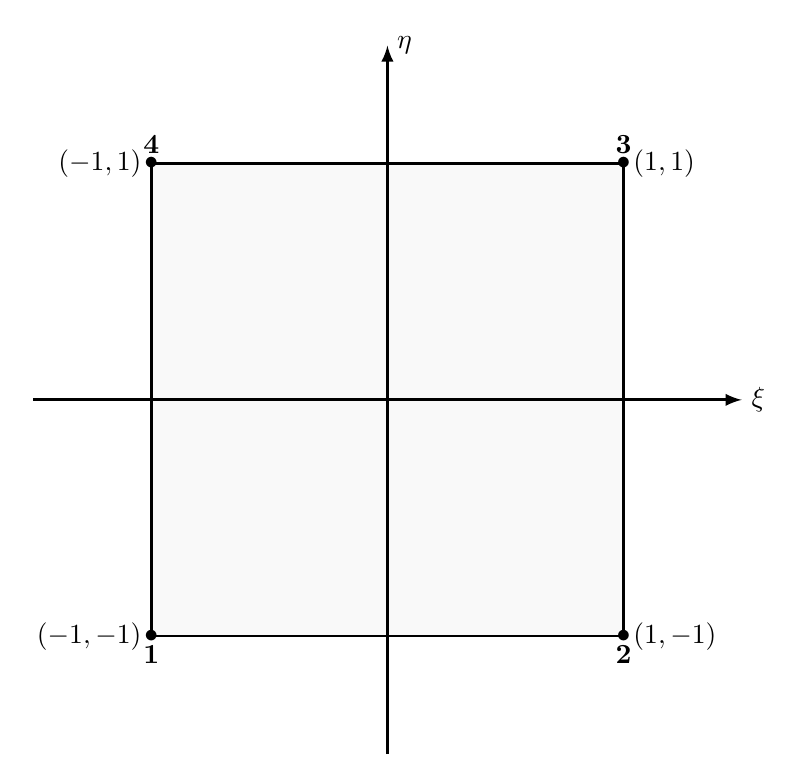
\begin{tikzpicture}[scale = 3.]
	\coordinate[](a) at (-1,-1);
	\coordinate[](b) at (1,-1);	
	\coordinate[](c) at (1,1);
	\coordinate[](d) at (-1,1);
	
	\coordinate[](aa) at (-1.5, 0);	
	\coordinate[](bb) at (1.5, 0);
	\coordinate[](cc) at (0,-1.5);
	\coordinate[](dd) at (0,1.5);

	% Element
	\filldraw[fill=gray!5!white, line width=1pt, draw=black] 
	(a) -- (b) -- (c) -- (d) -- cycle;
	\fill[black] node at (a) {$\bullet$};
	\fill[black] node at (b) {$\bullet$};
	\fill[black] node at (c) {$\bullet$};
	\fill[black] node at (d) {$\bullet$};	

	%% Axis
	\draw [->,line width=1.0pt,black] (aa) -- (bb);
	\draw [->,line width=1.0pt,black] (cc) -- (dd);
	\node[black,right] at (bb) {$\xi$};
	\node[black,right] at (dd) {$\eta$};
	
	%% Node numeration
	\node[black, below] at (a) {$\mathbf{1}$};
	\node[black, left] at (a) {$(-1,-1)$};
	%
	\node[black, below] at (b) {$\mathbf{2}$};
	\node[black, right] at (b) {$(1,-1)$};
	%
	\node[black, above] at (c) {$\mathbf{3}$};
	\node[black, right] at (c) {$(1,1)$};
	%
	\node[black, above] at (d) {$\mathbf{4}$};
	\node[black, left] at (d) {$(-1,1)$};
	
\end{tikzpicture}
%\end{center}
%\caption{Reference Element}
%\end{figure}
%
%\end{document}
\caption{Reference Element \label{fig:ref_element}}
\end{center}
\end{figure}
%
\begin{equation}
\begin{split}
&\phi_{1}=\frac{1}{4}(1-\xi)(1-\eta) \:, \:\:\:\: \phi_{2}=\frac{1}{4}(1+\xi)(1-\eta) \:,\\
&\phi_{3}=\frac{1}{4}(1+\xi)(1+\eta) \:, \:\:\:\: \phi_{4}=\frac{1}{4}(1-\xi)(1+\eta) \:.
\end{split}
\end{equation}   
and
\begin{equation}
\begin{split}
&\mu_{1} = 1 - 3\xi - 3\eta + 9\xi\eta \:, \:\:\:\: 
\mu_{2} = 1 + 3\xi - 3\eta - 9\xi\eta \:,\\
&\mu_{3} = 1 + 3\xi + 3\eta + 9\xi\eta \:, \:\:\:\: 
\mu_{4} = 1 - 3\xi + 3\eta + 9\xi\eta \:.
\end{split}
\end{equation}
It is important to observe that the global basis functions of the space $M_{h}$ are not continuous.
   
\subsection{Bubble functions}
In this section we detail the different choosing of the bubble functions. Addition of the bubble functions is essential to create a stable space. we have four types of bubbles.
In the first two cases we use a modification of the standard bubble function ,that is for the reference element:
\begin{equation}\label{eq:standard_bubble_fun}
b_{T}(\xi,\eta) = (1-\xi^{2})(1-\eta^{2})\:,
\end{equation}
while in the next two, we add to the standard bubble function another one.
\subsubsection{One Bubble function (type 1)}
As a first choice of bubble function we use:
\begin{equation}\label{eq:bubble_1}
\hat{b}_{T}(\xi,\eta) = c_{T}\cdot\phi_{T}(\xi,\eta)\cdot b_{T}(\xi,\eta)\:, 
\end{equation}
where $c_{T}$ is a coefficient in order to obtain $\hat{b}_{T}(\xi_{g},\eta_{g}) = 1$ (where $\bm{g}$ is the centroid of the elements), $\phi_{K}$ is the standard bilinear basis function corresponding to the lower-left corner of the square $T$.
In the case of reference square element we obtain:
\begin{equation} \label{eq:bubble_1_ref}
\hat{b}_{T}(\xi,\eta) = (1-\xi)(1-\eta)(1-\xi^{2})(1-\eta^{2})\:.
\end{equation}

\subsubsection{One Bubble function (type 2)}
The second choice of bubble function we take:
\begin{equation}\label{eq:bubble_2}
\hat{b}_{T}(\xi,\eta) = c_{T}\cdot (a+b\xi+c\eta)\cdot b_{T}(\xi,\eta)\:,
\end{equation}
where $a,b,c \in \mathrm{R}$ and $a,b,c \neq 0$.
For simplicity we set $a=b=c=1$ and we obtain for the reference square:
\begin{equation}\label{eq:bubble_2_ref}
\hat{b}_{T}(\xi,\eta) = (1+\xi+\eta)(1-\xi^{2})(1-\eta^{2})\:.
\end{equation} 

\subsubsection{Two Bubble functions}
Using two bubble functions, where the first is the standard bubble function and the second bubble is a modification of the standard bubble:
\begin{equation}\label{eq:bubble_3}
\begin{split}
&\hat{b}_{T1}(\xi,\eta) = b_{T}\:, \\
&\hat{b}_{T2}(\xi,\eta) = c_{T}\cdot (a\xi+b\eta)\cdot b_{T}\:,
\end{split}
\end{equation}
where $a,b \in \mathrm{R}$ and $a^{2}+b^{2}\neq 0$.
For the sake of simplicity we adopt $a=b=1$.
One obtains:
\begin{equation}\label{eq:bubble_3_ref}
\begin{split}
&\hat{b}_{T1}(\xi,\eta) = (1-\xi^{2})(1-\eta^{2})\:, \\
&\hat{b}_{T2}(\xi,\eta) = (\xi+\eta)(1-\xi^{2})(1-\eta^{2})\:.
\end{split}
\end{equation}

\subsubsection{Two Bubble functions, which one mixed}
As a finally choice of bubbles we use a standard bubble function plus one mixed bubble function for the two components of displacement.
\begin{equation}
\begin{split}
&\hat{b}_{T1}(\xi,\eta) = b_{T}\:, \\
&\hat{b}_{T2,\xi}(\xi,\eta) = (\nabla \phi_{1})_{\xi}\cdot b_{T}\:, \\
&\hat{b}_{T2,\eta}(\xi,\eta) = (\nabla \phi_{1})_{\eta}\cdot b_{T}\:,
\end{split}
\end{equation}
where $(\nabla\phi_{1})_{i}$ is $i$-th component of the gradient of the first shape function $\phi$.
In this way we have as shape function for the displacement using the mixed bubble function the vector $\left[\hat{b}_{T2,x}(x,y),\hat{b}_{T2,y}(x,y)\right]$. 

\section{Numerical example}\label{sec:five}
In this section we report some examples using the presented formulation to proven the good behaviour. 

\subsection{Square problem}
First example is a unit square domain with homogeneous Dirichlet boundary conditions. This benchmark problem is analyzed in \cite{brenner}.
The Lamé constant are fix to $\nu=0.49995$ and $\mu=1$.
We impose the body forces in using the following expressions:
$f$
\begin{equation}
\begin{split}
&f_{1} = \beta \left(\pi^{2} \left(4\sin\left(\pi y\right)
\left(-1+2\cos\left(2\pi x\right)\right)
-\cos\left(\pi\left(x+y\right)\right) \right.\right. \\
&\left.\left. \hspace{24pt} + A\sin\left(\pi x\right)\sin\left(\pi y\right)\right)\right)\:, \\
&f_{2} = \beta \left(\pi^{2}\left(4\sin\left(2\pi x\right)
\left(1-2\cos\left(2\pi y\right)\right)
-\cos\left(\pi\left(x+y\right)\right)\right.\right. \\
&\left.\left. \hspace{24pt} + A\sin\left(\pi x\right)\sin\left(\pi y\right)\right)\right)\:,
\end{split}
\end{equation}
where
\begin{equation}
A=\frac{2}{1+\lambda} \:\: \mbox{and} \:\: \beta =\frac{1}{25}\:.
\end{equation}
By imposition of the previously body forces the exact solution is:
\begin{equation} \label{eq:exact_solution}
\begin{split}
&u_{1} = \beta\left(\sin\left(2\pi y\right)
\left(-1+\cos\left(2\pi x\right)\right)+B\right)\:, \\
&u_{2} = \beta\left(\sin\left(2\pi x\right)
\left(1-\cos\left(2\pi y\right)\right)+B\right)\:,
\end{split}
\end{equation} 
where 
\begin{equation}
B=0.5A\sin\left(\pi x\right)\sin\left(\pi y\right)\:.
\end{equation}
The problem is study using two type of mesh: first of all using a square mesh and before using a trapezoidal mesh. The two types of mesh are shown in figures \ref{fig:square_regular} and \ref{fig:square_irregular}.
Figures \ref{fig:error_l2_1B_type1}, \ref{fig:error_l2_1B_type2}, \ref{fig:error_l2_2B} and \ref{fig:error_l2_2B_mixed} shown the error in norm $L^{2}$ in the case of regular mesh for the different types of bubble functions used and types of coefficient $\alpha$. All types of element converge in a good way.
In Figures  \ref{fig:error_dist_l2_1B_type1}, \ref{fig:error_dist_l2_1B_type2}, \ref{fig:error_dist_l2_2B} and \ref{fig:error_dist_l2_2B_mixed} we report the previously results in the case of trapezoidal meshes. 
%
\begin{figure}[h!]
\begin{center}
\subfigure[Regular mesh \label{fig:square_regular}]
{%\documentclass{article}
%
%\usepackage{tikz}
%\usepackage{tikz-3dplot}
%\usetikzlibrary{calc}
%\usetikzlibrary{patterns}
%\usetikzlibrary{intersections}
%\usetikzlibrary{arrows}
%\tikzset{>=latex}
%
%\begin{document}
%
%\begin{figure}[!h]
%\begin{center}

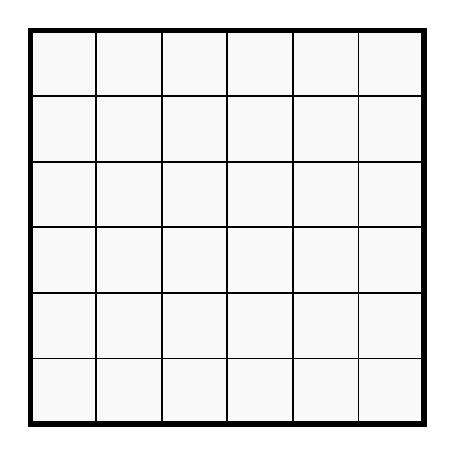
\begin{tikzpicture}[scale = 5.]
	\coordinate[](a) at (0,0);
	\coordinate[](b) at (1,0);	
	\coordinate[](c) at (1,1);
	\coordinate[](d) at (0,1);
	
	\pgfmathsetmacro{\h}{1}	
 	\pgfmathsetmacro{\dh}{1/6}
	
	% Trave
	\filldraw[fill=gray!5!white, line width=2pt, draw=black] 
	(a) -- (b) -- (c) -- (d) -- cycle;

	\begin{scope}[]
	\foreach \x in {1,2,...,5}
	{
	\draw[line width=0.7pt, draw=black] (\x*\dh,  0) -- (\x*\dh,\h);
	\draw[line width=0.7pt, draw=black] (0, \x*\dh) -- (\h, \x*\dh);
	}
	\end{scope}
		
\end{tikzpicture}
%\end{center}
%\caption{Square Problem (regular mesh)}
%\end{figure}
%
%\end{document}}
\hspace{5pt}
\subfigure[Trapezoidal mesh \label{fig:square_irregular}]{%\documentclass{article}
%
%\usepackage{tikz}
%\usepackage{tikz-3dplot}
%\usetikzlibrary{calc}
%\usetikzlibrary{patterns}
%\usetikzlibrary{intersections}
%\usetikzlibrary{arrows}
%\tikzset{>=latex}
%
%\begin{document}
%
%\begin{figure}[!h]
%\begin{center}

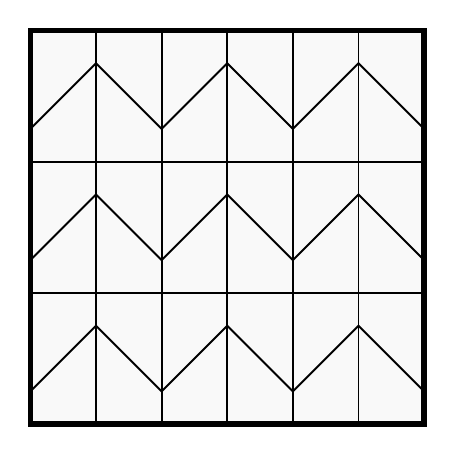
\begin{tikzpicture}[scale = 5.]
	\coordinate[](a) at (0,0);
	\coordinate[](b) at (1,0);	
	\coordinate[](c) at (1,1);
	\coordinate[](d) at (0,1);
	
	\pgfmathsetmacro{\h}{1}	
 	\pgfmathsetmacro{\dh}{1/6}
	
	% Trave
	\filldraw[fill=gray!5!white, line width=2pt, draw=black] 
	(a) -- (b) -- (c) -- (d) -- cycle;

	\begin{scope}[]
	\foreach \x in {1,3,...,5}
	{
	\draw[line width=0.7pt, draw=black] 
	(0, \x*\dh-\dh/2) -- (\dh, \x*\dh+\dh/2) -- (2*\dh, \x*\dh-\dh/2) -- 
	(3*\dh, \x*\dh+\dh/2) -- (4*\dh, \x*\dh-\dh/2) -- (5*\dh, \x*\dh+\dh/2)
	-- (6*\dh, \x*\dh-\dh/2);
	}
	\end{scope}
	
	\begin{scope}[]
	\foreach \x in {1,2,...,5}
	{
	\draw[line width=0.7pt, draw=black] (\x*\dh,  0) -- (\x*\dh,\h);
	}
	\end{scope}
	
	\begin{scope}[]
	\foreach \x in {2,4,...,5}
	{
	\draw[line width=0.7pt, draw=black] (0, \x*\dh) -- (\h, \x*\dh);
	}
	\end{scope}	
	
	
		
\end{tikzpicture}
%\end{center}
%\caption{Square Problem (irregular mesh)}
%\end{figure}
%
%\end{document}}
\caption{Square Problem}
\end{center}
\end{figure}
% Error L2
\begin{figure}[h!]
\begin{center}
\subfigure[type 1 \label{fig:error_l2_1B_type1}]
{%\documentclass{article}
%
%\usepackage{graphicx}
%\usepackage{xcolor}
%\usepackage{colortbl}
%\usepackage{fp}
%\usepackage{tikz, pgfplots}
%\usetikzlibrary{calc}
%\usetikzlibrary{patterns}
%\usetikzlibrary{intersections}
%\usetikzlibrary{arrows}
%\tikzset{>=latex}
%
%% Color definition
%\definecolor{green2}{RGB}{154, 205, 50}
%\definecolor{green3}{RGB}{141, 182, 0}
%\definecolor{blue2}{RGB}{0, 102, 255}
%\definecolor{lightgreen}{RGB}{178,255,102}
%
%
%\begin{document}
%\scriptsize
%\begin{figure}[!h]
%\begin{center}
\begin{tikzpicture}
 \begin{loglogaxis}[width=0.45\textwidth, height=0.45\textwidth,
  legend style={anchor=south, at={(0.5, 1.07)}, draw=none, font=\scriptsize},
  grid=major,
  legend columns=3, transpose legend,
  xlabel={Number of Elements},
  ylabel={$\left(\parallel u_{h}-u \parallel_{L^{2}}\right)/ \parallel u \parallel_{L^{2}}$},
  xmin=10, xmax=1e4,
  ymin=1e-3, ymax=1e0,
  ytick={1e-3, 1e-2, 1e-1, 1},
  yticklabels={$10^{-3}$, $10^{-2}$, $10^{-1}$, $10^{0}$},
  xtick={1e1, 1e2, 1e3, 1e4},
  xticklabels={$10^{1}$, $10^{2}$, $10^{3}$, $10^{4}$},
 ]
 % Reference
 %\addplot[black, ultra thick] coordinates{
 %(50, 1.8248e-5)
 %(15000, 1.8248e-5)
 %}; 
 %\addlegendentry{Reference} 
 %
 \addplot[red, mark=+, thick, mark options={solid}]
 table [x index={0}, y index={1}]
 {square_example/bolla1_type1/elastic_error_disp_u_l2_lmu1.txt};
 \addlegendentry{$\alpha / \mu=1$}
 %
 \addplot[blue, mark=x, thick, mark options={solid}]
 table [x index={0}, y index={1}]
 {square_example/bolla1_type1/elastic_error_disp_u_l2_lmu2.txt};
 \addlegendentry{$\alpha / \mu=2$}
 %
 \addplot[green3, mark=o, thick, mark options={solid}]
 table [x index={0}, y index={1}]
 {square_example/bolla1_type1/elastic_error_disp_u_l2_lmu3.txt};
 \addlegendentry{$\alpha / \mu=3$}
 %
 %\addplot[red, mark=+, dashed, very thick]
 %table [x index={0}, y index={1}]
 %{};
 %\addlegendentry{}
 %
 %\addplot[blue, mark=x, very thick]
 %table [x index={0}, y index={1}]
 %{};
 %\addlegendentry{}
 %
 %\addplot[green3, mark=x, very thick]
 %table [x index={0}, y index={1}]
 %{};
 %\addlegendentry{}
 % 
 \end{loglogaxis}
\end{tikzpicture}
%\end{center}
%\caption{The relative error versus the number of elements measured relative 
%to the $L^{2}$}
%\end{figure}
%
%\end{document}
}
\subfigure[type 2 \label{fig:error_l2_1B_type2}]
{%\documentclass{article}
%
%\usepackage{graphicx}
%\usepackage{xcolor}
%\usepackage{colortbl}
%\usepackage{fp}
%\usepackage{tikz, pgfplots}
%\usetikzlibrary{calc}
%\usetikzlibrary{patterns}
%\usetikzlibrary{intersections}
%\usetikzlibrary{arrows}
%\tikzset{>=latex}
%
%% Color definition
%\definecolor{green2}{RGB}{154, 205, 50}
%\definecolor{green3}{RGB}{141, 182, 0}
%\definecolor{blue2}{RGB}{0, 102, 255}
%\definecolor{lightgreen}{RGB}{178,255,102}
%
%
%\begin{document}
%\scriptsize
%\begin{figure}[!h]
%\begin{center}
\begin{tikzpicture}
 \begin{loglogaxis}[width=0.45\textwidth, height=0.45\textwidth,
  legend style={anchor=south, at={(0.5, 1.07)}, draw=none, font=\scriptsize},
  grid=major,
  legend columns=3, transpose legend,
  xlabel={Number of Elements},
  ylabel={$\left(\parallel u_{h}-u \parallel_{L^{2}}\right)/ \parallel u \parallel_{L^{2}}$},
  xmin=10, xmax=1e4,
  ymin=1e-3, ymax=1e0,
  ytick={1e-3, 1e-2, 1e-1, 1},
  yticklabels={$10^{-3}$, $10^{-2}$, $10^{-1}$, $10^{0}$},
  xtick={1e1, 1e2, 1e3, 1e4},
  xticklabels={$10^{1}$, $10^{2}$, $10^{3}$, $10^{4}$},
 ]
 % Reference
 %\addplot[black, ultra thick] coordinates{
 %(50, 1.8248e-5)
 %(15000, 1.8248e-5)
 %}; 
 %\addlegendentry{Reference} 
 %
 \addplot[red, mark=+, thick, mark options={solid}]
 table [x index={0}, y index={1}]
 {square_example/bolla1_type1/elastic_error_disp_u_l2_lmu1.txt};
 \addlegendentry{$\alpha / \mu=1$}
 %
 \addplot[blue, mark=x, thick, mark options={solid}]
 table [x index={0}, y index={1}]
 {square_example/bolla1_type1/elastic_error_disp_u_l2_lmu2.txt};
 \addlegendentry{$\alpha / \mu=2$}
 %
 \addplot[green3, mark=o, thick, mark options={solid}]
 table [x index={0}, y index={1}]
 {square_example/bolla1_type1/elastic_error_disp_u_l2_lmu3.txt};
 \addlegendentry{$\alpha / \mu=3$}
 %
 %\addplot[red, mark=+, dashed, very thick]
 %table [x index={0}, y index={1}]
 %{};
 %\addlegendentry{}
 %
 %\addplot[blue, mark=x, very thick]
 %table [x index={0}, y index={1}]
 %{};
 %\addlegendentry{}
 %
 %\addplot[green3, mark=x, very thick]
 %table [x index={0}, y index={1}]
 %{};
 %\addlegendentry{}
 % 
 \end{loglogaxis}
\end{tikzpicture}
%\end{center}
%\caption{The relative error versus the number of elements measured relative 
%to the $L^{2}$}
%\end{figure}
%
%\end{document}
}
\caption{The relative error vs. the number of elements measured relative 
to the $L^{2}$ norm (Case one bubble function and regular mesh)}
\end{center}
\end{figure}
%
\begin{figure}[h!]
\begin{center}
\subfigure[Case two bubble function \label{fig:error_l2_2B}]{%\documentclass{article}
%
%\usepackage{graphicx}
%\usepackage{xcolor}
%\usepackage{colortbl}
%\usepackage{fp}
%\usepackage{tikz, pgfplots}
%\usetikzlibrary{calc}
%\usetikzlibrary{patterns}
%\usetikzlibrary{intersections}
%\usetikzlibrary{arrows}
%\tikzset{>=latex}
%
%% Color definition
%\definecolor{green2}{RGB}{154, 205, 50}
%\definecolor{green3}{RGB}{141, 182, 0}
%\definecolor{blue2}{RGB}{0, 102, 255}
%\definecolor{lightgreen}{RGB}{178,255,102}
%
%
%\begin{document}
%\begin{figure}[!h]
%\begin{center}
\begin{tikzpicture}
 %transpose legend
 \begin{loglogaxis}[width=0.45\textwidth, height=0.45\textwidth,
  legend style={anchor=south, at={(0.5, 1.07)}, draw=none, font=\scriptsize},
  grid=major,
  legend columns=3,
  xlabel={\large Number of Elements},
  ylabel={\Large $\frac{\parallel u_{h}-u \parallel_{L^{2}}}{\parallel u \parallel_{L^{2}}}$},
  xmin=1, xmax=1e4,
  ymin=1e-3, ymax=1e0,
  ytick={1e-3, 1e-2, 1e-1, 1},
  yticklabels={$10^{-3}$, $10^{-2}$, $10^{-1}$, $10^{0}$},
  xtick={1e0, 1e1, 1e2, 1e3, 1e4},
  xticklabels={$10^{0}$, $10^{1}$, $10^{2}$, $10^{3}$, $10^{4}$},
 ]
 % Reference
 %\addplot[black, ultra thick] coordinates{
 %(50, 1.8248e-5)
 %(15000, 1.8248e-5)
 %}; 
 %\addlegendentry{Reference} 
 %
 \addplot[red, mark=+, thick, mark options={solid}]
 table [x index={0}, y index={1}]
 {beam_example/regular/bolla2/error_beam_u_l2_1mu.txt};
 \addlegendentry{$\alpha / \mu=1$}
 %
 \addplot[blue, mark=x, thick, mark options={solid}]
 table [x index={0}, y index={1}]
 {beam_example/regular/bolla2/error_beam_u_l2_2mu.txt};
 \addlegendentry{$\alpha / \mu=2$}
 %
 \addplot[green3, mark=o, thick, mark options={solid}]
 table [x index={0}, y index={1}]
 {beam_example/regular/bolla2/error_beam_u_l2_3mu.txt};
 \addlegendentry{$\alpha / \mu=3$}
 %
 %\addplot[red, mark=+, very thick]
 %table [x index={0}, y index={1}]
 %{};
 %\addlegendentry{}
 %
 %\addplot[blue, mark=x, very thick]
 %table [x index={0}, y index={1}]
 %{};
 %\addlegendentry{}
 %
 %\addplot[green3, mark=x, very thick]
 %table [x index={0}, y index={1}]
 %{};
 %\addlegendentry{}
 % 
 \end{loglogaxis}
\end{tikzpicture}
%\end{center}
%\caption{The relative error versus the number of elements measured relative 
%to the $L^{2}$}
%\end{figure}
%
%\end{document}}
\subfigure[Case two bubble function of which one mixed \label{fig:error_l2_2B_mixed}]{%\documentclass{article}
%
%\usepackage{graphicx}
%\usepackage{xcolor}
%\usepackage{colortbl}
%\usepackage{fp}
%\usepackage{tikz, pgfplots}
%\usetikzlibrary{calc}
%\usetikzlibrary{patterns}
%\usetikzlibrary{intersections}
%\usetikzlibrary{arrows}
%\tikzset{>=latex}
%
%% Color definition
%\definecolor{green2}{RGB}{154, 205, 50}
%\definecolor{green3}{RGB}{141, 182, 0}
%\definecolor{blue2}{RGB}{0, 102, 255}
%\definecolor{lightgreen}{RGB}{178,255,102}
%
%
%\begin{document}
%\begin{figure}[!h]
%\begin{center}
\begin{tikzpicture}
 %transpose legend
 \begin{loglogaxis}[width=0.45\textwidth, height=0.45\textwidth,
  legend style={anchor=south, at={(0.5, 1.07)}, draw=none, font=\scriptsize},
  grid=major,
  legend columns=3,
  xlabel={Number of Elements},
  ylabel={$\frac{\parallel u_{h}-u \parallel_{L^{2}}}{\parallel u \parallel_{L^{2}}}$},
  xmin=1, xmax=1e4,
  ymin=1e-3, ymax=1e0,
  ytick={1e-3, 1e-2, 1e-1, 1},
  yticklabels={$10^{-3}$, $10^{-2}$, $10^{-1}$, $10^{0}$},
  xtick={1e0, 1e1, 1e2, 1e3, 1e4},
  xticklabels={$10^{0}$, $10^{1}$, $10^{2}$, $10^{3}$, $10^{4}$},
 ]
 % Reference
 %\addplot[black, ultra thick] coordinates{
 %(50, 1.8248e-5)
 %(15000, 1.8248e-5)
 %}; 
 %\addlegendentry{Reference} 
 %
 \addplot[red, mark=+, thick, mark options={solid}]
 table [x index={0}, y index={1}]
 {beam_example/regular/bolla2_mixed/error_beam_u_l2_1mu.txt};
 \addlegendentry{$\alpha / \mu=1$}
 %
 \addplot[blue, mark=x, thick, mark options={solid}]
 table [x index={0}, y index={1}]
 {beam_example/regular/bolla2_mixed/error_beam_u_l2_2mu.txt};
 \addlegendentry{$\alpha / \mu=2$}
 %
 \addplot[green3, mark=o, thick, mark options={solid}]
 table [x index={0}, y index={1}]
 {beam_example/regular/bolla2_mixed/error_beam_u_l2_3mu.txt};
 \addlegendentry{$\alpha / \mu=3$}
 %
 %\addplot[red, mark=+, very thick]
 %table [x index={0}, y index={1}]
 %{};
 %\addlegendentry{}
 %
 %\addplot[blue, mark=x, very thick]
 %table [x index={0}, y index={1}]
 %{};
 %\addlegendentry{}
 %
 %\addplot[green3, mark=x, very thick]
 %table [x index={0}, y index={1}]
 %{};
 %\addlegendentry{}
 % 
 \end{loglogaxis}
\end{tikzpicture}
%\end{center}
%\caption{The relative error versus the number of elements measured relative 
%to the $L^{2}$}
%\end{figure}
%
%\end{document}
}
\caption{The relative error versus the number of elements measured relative to the $L^{2}$ norm (regular mesh)}
\end{center}
\end{figure}
% Error L2 (Distorted)
\begin{figure}[h!]
\begin{center}
\subfigure[type 1 \label{fig:error_dist_l2_1B_type1}]
{%\documentclass{article}
%
%\usepackage{graphicx}
%\usepackage{xcolor}
%\usepackage{colortbl}
%\usepackage{fp}
%\usepackage{tikz, pgfplots}
%\usetikzlibrary{calc}
%\usetikzlibrary{patterns}
%\usetikzlibrary{intersections}
%\usetikzlibrary{arrows}
%\tikzset{>=latex}
%
%% Color definition
%\definecolor{green2}{RGB}{154, 205, 50}
%\definecolor{green3}{RGB}{141, 182, 0}
%\definecolor{blue2}{RGB}{0, 102, 255}
%\definecolor{lightgreen}{RGB}{178,255,102}
%
%
%\begin{document}
%
%\begin{figure}[!h]
%\begin{center}
\begin{tikzpicture}
 \begin{loglogaxis}[width=0.45\textwidth, height=0.45\textwidth,
  legend style={anchor=south, at={(0.5, 1.07)}, draw=none, font=\scriptsize},
  grid=major,
  legend columns=3, transpose legend,
  xlabel={Number of Elements},
  ylabel={$\left(\parallel u_{h}-u \parallel_{L^{2}}\right)/ \parallel u \parallel_{L^{2}}$},
  xmin=10, xmax=1e5,
  ymin=1e-3, ymax=1e0,
  ytick={1e-3, 1e-2, 1e-1, 1},
  yticklabels={$10^{-3}$, $10^{-2}$, $10^{-1}$, $10^{0}$},
  xtick={1e1, 1e2, 1e3, 1e4, 1e5},
  xticklabels={$10^{1}$, $10^{2}$, $10^{3}$, $10^{4}$, $10^{5}$},
 ]
 % Reference
 %\addplot[black, ultra thick] coordinates{
 %(50, 1.8248e-5)
 %(15000, 1.8248e-5)
 %}; 
 %\addlegendentry{Reference} 
 %
 \addplot[red, mark=+, thick, mark options={solid}]
 table [x index={0}, y index={1}]
 {square_example/bolla1_type2/elastic_error_dist_type_2_disp_u_l2_1mu.txt};
 \addlegendentry{$\alpha / \mu=1$}
 %
 \addplot[blue, mark=x, thick, mark options={solid}]
 table [x index={0}, y index={1}]
 {square_example/bolla1_type2/elastic_error_dist_type_2_disp_u_l2_2mu.txt};
 \addlegendentry{$\alpha / \mu=2$}
 %
 \addplot[green3, mark=o, thick, mark options={solid}]
 table [x index={0}, y index={1}]
 {square_example/bolla1_type2/elastic_error_dist_type_2_disp_u_l2_3mu.txt};
 \addlegendentry{$\alpha / \mu=3$}
 %
 %\addplot[red, mark=+, very thick]
 %table [x index={0}, y index={1}]
 %{};
 %\addlegendentry{}
 %
 %\addplot[blue, mark=x, very thick]
 %table [x index={0}, y index={1}]
 %{};
 %\addlegendentry{}
 %
 %\addplot[green3, mark=x, very thick]
 %table [x index={0}, y index={1}]
 %{};
 %\addlegendentry{}
 % 
 \end{loglogaxis}
\end{tikzpicture}
%\end{center}
%\caption{The relative error versus the number of elements measured relative 
%to the $L^{2}$}
%\end{figure}
%
%\end{document}
}
\subfigure[type 2 \label{fig:error_dist_l2_1B_type2}]
{%\documentclass{article}
%
%\usepackage{graphicx}
%\usepackage{xcolor}
%\usepackage{colortbl}
%\usepackage{fp}
%\usepackage{tikz, pgfplots}
%\usetikzlibrary{calc}
%\usetikzlibrary{patterns}
%\usetikzlibrary{intersections}
%\usetikzlibrary{arrows}
%\tikzset{>=latex}
%
%% Color definition
%\definecolor{green2}{RGB}{154, 205, 50}
%\definecolor{green3}{RGB}{141, 182, 0}
%\definecolor{blue2}{RGB}{0, 102, 255}
%\definecolor{lightgreen}{RGB}{178,255,102}
%
%
%\begin{document}
%
%\begin{figure}[!h]
%\begin{center}
\begin{tikzpicture}
 \begin{loglogaxis}[width=0.45\textwidth, height=0.45\textwidth,
  legend style={anchor=south, at={(0.5, 1.07)}, draw=none, font=\scriptsize},
  grid=major,
  legend columns=3, transpose legend,
  xlabel={Number of Elements},
  ylabel={$\left(\parallel u_{h}-u \parallel_{L^{2}}\right)/ \parallel u \parallel_{L^{2}}$},
  xmin=10, xmax=1e5,
  ymin=1e-3, ymax=1e0,
  ytick={1e-3, 1e-2, 1e-1, 1},
  yticklabels={$10^{-3}$, $10^{-2}$, $10^{-1}$, $10^{0}$},
  xtick={1e1, 1e2, 1e3, 1e4, 1e5},
  xticklabels={$10^{1}$, $10^{2}$, $10^{3}$, $10^{4}$, $10^{5}$},
 ]
 % Reference
 %\addplot[black, ultra thick] coordinates{
 %(50, 1.8248e-5)
 %(15000, 1.8248e-5)
 %}; 
 %\addlegendentry{Reference} 
 %
 \addplot[red, mark=+, thick, mark options={solid}]
 table [x index={0}, y index={1}]
 {square_example/bolla1_type2/elastic_error_dist_type_2_disp_u_l2_1mu.txt};
 \addlegendentry{$\alpha / \mu=1$}
 %
 \addplot[blue, mark=x, thick, mark options={solid}]
 table [x index={0}, y index={1}]
 {square_example/bolla1_type2/elastic_error_dist_type_2_disp_u_l2_2mu.txt};
 \addlegendentry{$\alpha / \mu=2$}
 %
 \addplot[green3, mark=o, thick, mark options={solid}]
 table [x index={0}, y index={1}]
 {square_example/bolla1_type2/elastic_error_dist_type_2_disp_u_l2_3mu.txt};
 \addlegendentry{$\alpha / \mu=3$}
 %
 %\addplot[red, mark=+, very thick]
 %table [x index={0}, y index={1}]
 %{};
 %\addlegendentry{}
 %
 %\addplot[blue, mark=x, very thick]
 %table [x index={0}, y index={1}]
 %{};
 %\addlegendentry{}
 %
 %\addplot[green3, mark=x, very thick]
 %table [x index={0}, y index={1}]
 %{};
 %\addlegendentry{}
 % 
 \end{loglogaxis}
\end{tikzpicture}
%\end{center}
%\caption{The relative error versus the number of elements measured relative 
%to the $L^{2}$}
%\end{figure}
%
%\end{document}
}
\caption{The relative error vs. the number of elements measured relative 
to the $L^{2}$ norm (Case one bubble function and Trapezoidal mesh)}
\end{center}
\end{figure}
%
\begin{figure}[h!]
\begin{center}
\subfigure[Case two bubble function \label{fig:error_dist_l2_2B}]
{%\documentclass{article}
%
%\usepackage{graphicx}
%\usepackage{xcolor}
%\usepackage{colortbl}
%\usepackage{fp}
%\usepackage{tikz, pgfplots}
%\usetikzlibrary{calc}
%\usetikzlibrary{patterns}
%\usetikzlibrary{intersections}
%\usetikzlibrary{arrows}
%\tikzset{>=latex}
%
%% Color definition
%\definecolor{green2}{RGB}{154, 205, 50}
%\definecolor{green3}{RGB}{141, 182, 0}
%\definecolor{blue2}{RGB}{0, 102, 255}
%\definecolor{lightgreen}{RGB}{178,255,102}
%
%
%\begin{document}
%
%\begin{figure}[!h]
%\begin{center}
\begin{tikzpicture}
 %transpose legend
 \begin{loglogaxis}[width=0.45\textwidth, height=0.45\textwidth,
  legend style={anchor=south, at={(0.5, 1.07)}, draw=none, font=\scriptsize},
  grid=major,
  legend columns=3,
  xlabel={\large Number of Elements},
  ylabel={\Large $\frac{\parallel u_{h}-u \parallel_{L^{2}}}{\parallel u \parallel_{L^{2}}}$},
  xmin=10, xmax=1e5,
  ymin=1e-3, ymax=1e0,
  ytick={1e-3, 1e-2, 1e-1, 1},
  yticklabels={$10^{-3}$, $10^{-2}$, $10^{-1}$, $10^{0}$},
  xtick={1e1, 1e2, 1e3, 1e4, 1e5},
  xticklabels={$10^{1}$, $10^{2}$, $10^{3}$, $10^{4}$, $10^{5}$},
 ]
 % Reference
 %\addplot[black, ultra thick] coordinates{
 %(50, 1.8248e-5)
 %(15000, 1.8248e-5)
 %}; 
 %\addlegendentry{Reference} 
 %
 \addplot[red, mark=+, thick, mark options={solid}]
 table [x index={0}, y index={1}]
 {square_example/bolla2/elastic_error_dist_disp_u_l2_1mu.txt};
 \addlegendentry{$\alpha / \mu=1$}
 %
 \addplot[blue, mark=x, thick, mark options={solid}]
 table [x index={0}, y index={1}]
 {square_example/bolla2/elastic_error_dist_disp_u_l2_2mu.txt};
 \addlegendentry{$\alpha / \mu=2$}
 %
 \addplot[green3, mark=o, thick, mark options={solid}]
 table [x index={0}, y index={1}]
 {square_example/bolla2/elastic_error_dist_disp_u_l2_3mu.txt};
 \addlegendentry{$\alpha / \mu=3$}
 %
 %\addplot[red, mark=+, very thick]
 %table [x index={0}, y index={1}]
 %{};
 %\addlegendentry{}
 %
 %\addplot[blue, mark=x, very thick]
 %table [x index={0}, y index={1}]
 %{};
 %\addlegendentry{}
 %
 %\addplot[green3, mark=x, very thick]
 %table [x index={0}, y index={1}]
 %{};
 %\addlegendentry{}
 % 
 \end{loglogaxis}
\end{tikzpicture}
%\end{center}
%\caption{The relative error versus the number of elements measured relative 
%to the $L^{2}$}
%\end{figure}
%
%\end{document}
}
\subfigure[Case two bubble function of which one mixed \label{fig:error_dist_l2_2B_mixed}]
{%\documentclass{article}
%
%\usepackage{graphicx}
%\usepackage{xcolor}
%\usepackage{colortbl}
%\usepackage{fp}
%\usepackage{tikz, pgfplots}
%\usetikzlibrary{calc}
%\usetikzlibrary{patterns}
%\usetikzlibrary{intersections}
%\usetikzlibrary{arrows}
%\tikzset{>=latex}
%
%% Color definition
%\definecolor{green2}{RGB}{154, 205, 50}
%\definecolor{green3}{RGB}{141, 182, 0}
%\definecolor{blue2}{RGB}{0, 102, 255}
%\definecolor{lightgreen}{RGB}{178,255,102}
%
%
%\begin{document}
%
%\begin{figure}[!h]
%\begin{center}
\begin{tikzpicture}
 %transpose legend
 \begin{loglogaxis}[width=0.45\textwidth, height=0.45\textwidth,
  legend style={anchor=south, at={(0.5, 1.07)}, draw=none, font=\scriptsize},
  grid=major,
  legend columns=3,
  xlabel={\large Number of Elements},
  ylabel={\Large $\frac{\parallel u_{h}-u \parallel_{L^{2}}}{\parallel u \parallel_{L^{2}}}$},
  xmin=10, xmax=1e5,
  ymin=1e-3, ymax=1e0,
  ytick={1e-3, 1e-2, 1e-1, 1},
  yticklabels={$10^{-3}$, $10^{-2}$, $10^{-1}$, $10^{0}$},
  xtick={1e1, 1e2, 1e3, 1e4, 1e5},
  xticklabels={$10^{1}$, $10^{2}$, $10^{3}$, $10^{4}$,$10^{5}$},
 ]
 % Reference
 %\addplot[black, ultra thick] coordinates{
 %(50, 1.8248e-5)
 %(15000, 1.8248e-5)
 %}; 
 %\addlegendentry{Reference} 
 %
 \addplot[red, mark=+, thick, mark options={solid}]
 table [x index={0}, y index={1}]
 {square_example/bolla2_mixed/elastic_error_dist_disp_u_l2_1mu.txt};
 \addlegendentry{$\alpha / \mu=1$}
 %
 \addplot[blue, mark=x, thick, mark options={solid}]
 table [x index={0}, y index={1}]
 {square_example/bolla2_mixed/elastic_error_dist_disp_u_l2_2mu.txt};
 \addlegendentry{$\alpha / \mu=2$}
 %
 \addplot[green3, mark=o, thick, mark options={solid}]
 table [x index={0}, y index={1}]
 {square_example/bolla2_mixed/elastic_error_dist_disp_u_l2_3mu.txt};
 \addlegendentry{$\alpha / \mu=3$}
 
% \addplot[red, mark=+, very thick]
% table [x index={0}, y index={1}]
% {square_example/bolla2_mixed/elastic_error_dist_disp_u_l2_lmu1.txt};
% \addlegendentry{Dist $\alpha / \mu=1$}
 %
 %\addplot[blue, mark=x, very thick]
 %table [x index={0}, y index={1}]
 %{};
 %\addlegendentry{}
 %
 %\addplot[green3, mark=x, very thick]
 %table [x index={0}, y index={1}]
 %{};
 %\addlegendentry{}
 % 
 \end{loglogaxis}
\end{tikzpicture}
%\end{center}
%\caption{The relative error versus the number of elements measured relative 
%to the $L^{2}$}
%\end{figure}
%
%\end{document}
}
\caption{The relative error vs. the number of elements measured relative 
to the $L^{2}$ norm (Case one bubble function and Trapezoidal mesh)}
\end{center}
\end{figure}
%
% Strain
\begin{figure}[h!]
\begin{center}
\subfigure[Case regular mesh \label{fig:error_strain_xx_l2_2B}]
{%\documentclass{article}
%
%\usepackage{graphicx}
%\usepackage{xcolor}
%\usepackage{colortbl}
%\usepackage{fp}
%\usepackage{tikz, pgfplots}
%\usetikzlibrary{calc}
%\usetikzlibrary{patterns}
%\usetikzlibrary{intersections}
%\usetikzlibrary{arrows}
%\tikzset{>=latex}
%
%% Color definition
%\definecolor{green2}{RGB}{154, 205, 50}
%\definecolor{green3}{RGB}{141, 182, 0}
%\definecolor{blue2}{RGB}{0, 102, 255}
%\definecolor{lightgreen}{RGB}{178,255,102}
%
%
%\begin{document}
%
%\begin{figure}[!h]
%\begin{center}
\begin{tikzpicture}
 %transpose legend
 \begin{loglogaxis}[width=0.45\textwidth, height=0.45\textwidth,
  legend style={anchor=south, at={(0.5, 1.07)}, draw=none, font=\scriptsize},
  grid=major,
  legend columns=3,
  xlabel={\large Number of Elements},
  ylabel={\Large $\frac{\parallel d_{h}-d \parallel_{L^{2}}}{\parallel d \parallel_{L^{2}}}$},
  xmin=10, xmax=1e4,
  ymin=1e-3, ymax=1e0,
  ytick={1e-3, 1e-2, 1e-1, 1},
  yticklabels={$10^{-3}$, $10^{-2}$, $10^{-1}$, $10^{0}$},
  xtick={1e1, 1e2, 1e3, 1e4},
  xticklabels={$10^{1}$, $10^{2}$, $10^{3}$, $10^{4}$},
 ]
 % Reference
 %\addplot[black, ultra thick] coordinates{
 %(50, 1.8248e-5)
 %(15000, 1.8248e-5)
 %}; 
 %\addlegendentry{Reference} 
 %
 \addplot[red, mark=+, thick, mark options={solid}]
 table [x index={0}, y index={1}]
 {square_example/bolla2/elastic_error_l2_strain_xx_2B_1mu.txt};
 \addlegendentry{$\alpha / \mu=1$}
 %
 \addplot[blue, mark=x, thick, mark options={solid}]
 table [x index={0}, y index={1}]
 {square_example/bolla2/elastic_error_l2_strain_xx_2B_2mu.txt};
 \addlegendentry{$\alpha / \mu=2$}
 %
 \addplot[green3, mark=o, thick, mark options={solid}]
 table [x index={0}, y index={1}]
 {square_example/bolla2/elastic_error_l2_strain_xx_2B_3mu.txt};
 \addlegendentry{$\alpha / \mu=3$}
 %
 %\addplot[red, mark=+, very thick]
 %table [x index={0}, y index={1}]
 %{};
 %\addlegendentry{}
 %
 %\addplot[blue, mark=x, very thick]
 %table [x index={0}, y index={1}]
 %{};
 %\addlegendentry{}
 %
 %\addplot[green3, mark=x, very thick]
 %table [x index={0}, y index={1}]
 %{};
 %\addlegendentry{}
 % 
 \end{loglogaxis}
\end{tikzpicture}
%\end{center}
%\caption{The relative error versus the number of elements measured relative 
%to the $L^{2}$}
%\end{figure}
%
%\end{document}
}
\subfigure[Case trapezoidal mesh \label{fig:error_strain_xx_l2_2B_dist}]
{%\documentclass{article}
%
%\usepackage{graphicx}
%\usepackage{xcolor}
%\usepackage{colortbl}
%\usepackage{fp}
%\usepackage{tikz, pgfplots}
%\usetikzlibrary{calc}
%\usetikzlibrary{patterns}
%\usetikzlibrary{intersections}
%\usetikzlibrary{arrows}
%\tikzset{>=latex}
%
%% Color definition
%\definecolor{green2}{RGB}{154, 205, 50}
%\definecolor{green3}{RGB}{141, 182, 0}
%\definecolor{blue2}{RGB}{0, 102, 255}
%\definecolor{lightgreen}{RGB}{178,255,102}
%
%
%\begin{document}
%
%\begin{figure}[!h]
%\begin{center}
\begin{tikzpicture}
 %transpose legend
 \begin{loglogaxis}[width=0.45\textwidth, height=0.45\textwidth,
  legend style={anchor=south, at={(0.5, 1.07)}, draw=none, font=\scriptsize},
  grid=major,
  legend columns=3,
  xlabel={\large Number of Elements},
  ylabel={\Large $\frac{\parallel d_{h}-d \parallel_{L^{2}}}{\parallel d \parallel_{L^{2}}}$},
  xmin=10, xmax=1e4,
  ymin=1e-3, ymax=1e0,
  ytick={1e-3, 1e-2, 1e-1, 1},
  yticklabels={$10^{-3}$, $10^{-2}$, $10^{-1}$, $10^{0}$},
  xtick={1e1, 1e2, 1e3, 1e4},
  xticklabels={$10^{1}$, $10^{2}$, $10^{3}$, $10^{4}$},
 ]
 % Reference
 %\addplot[black, ultra thick] coordinates{
 %(50, 1.8248e-5)
 %(15000, 1.8248e-5)
 %}; 
 %\addlegendentry{Reference} 
 %
 \addplot[red, mark=+, thick, mark options={solid}]
 table [x index={0}, y index={1}]
 {square_example/bolla2/elastic_error_l2_strain_xx_2B_dist_1mu.txt};
 \addlegendentry{$\alpha / \mu=1$}
 %
 \addplot[blue, mark=x, thick, mark options={solid}]
 table [x index={0}, y index={1}]
 {square_example/bolla2/elastic_error_l2_strain_xx_2B_dist_2mu.txt};
 \addlegendentry{$\alpha / \mu=2$}
 %
 \addplot[green3, mark=o, thick, mark options={solid}]
 table [x index={0}, y index={1}]
 {square_example/bolla2/elastic_error_l2_strain_xx_2B_dist_3mu.txt};
 \addlegendentry{$\alpha / \mu=3$}
 %
 %\addplot[red, mark=+, very thick]
 %table [x index={0}, y index={1}]
 %{};
 %\addlegendentry{}
 %
 %\addplot[blue, mark=x, very thick]
 %table [x index={0}, y index={1}]
 %{};
 %\addlegendentry{}
 %
 %\addplot[green3, mark=x, very thick]
 %table [x index={0}, y index={1}]
 %{};
 %\addlegendentry{}
 % 
 \end{loglogaxis}
\end{tikzpicture}
%\end{center}
%\caption{The relative error versus the number of elements measured relative 
%to the $L^{2}$}
%\end{figure}
%
%\end{document}
}
\caption{The relative error of strain $\bm{d}_{xx}$ vs. 
the number of elements (Case of two bubble functions)}
\end{center}
\end{figure}
%
\begin{figure}[h!]
\begin{center}
\subfigure[Case regular mesh \label{fig:error_strain_xx_l2_2B_mixed}]
{%\documentclass{article}
%
%\usepackage{graphicx}
%\usepackage{xcolor}
%\usepackage{colortbl}
%\usepackage{fp}
%\usepackage{tikz, pgfplots}
%\usetikzlibrary{calc}
%\usetikzlibrary{patterns}
%\usetikzlibrary{intersections}
%\usetikzlibrary{arrows}
%\tikzset{>=latex}
%
%% Color definition
%\definecolor{green2}{RGB}{154, 205, 50}
%\definecolor{green3}{RGB}{141, 182, 0}
%\definecolor{blue2}{RGB}{0, 102, 255}
%\definecolor{lightgreen}{RGB}{178,255,102}
%
%
%\begin{document}
%
%\begin{figure}[!h]
%\begin{center}
\begin{tikzpicture}
 \begin{loglogaxis}[width=0.45\textwidth, height=0.45\textwidth,
  legend style={anchor=south, at={(0.5, 1.07)}, draw=none, font=\scriptsize},
  grid=major,
  legend columns=3, transpose legend,
  xlabel={Number of Elements},
  ylabel={$\left(\parallel d_{h}-d \parallel_{L^{2}}\right)/ \parallel d \parallel_{L^{2}}$},
  xmin=10, xmax=1e4,
  ymin=1e-3, ymax=1e0,
  ytick={1e-3, 1e-2, 1e-1, 1},
  yticklabels={$10^{-3}$, $10^{-2}$, $10^{-1}$, $10^{0}$},
  xtick={1e1, 1e2, 1e3, 1e4},
  xticklabels={$10^{1}$, $10^{2}$, $10^{3}$, $10^{4}$},
 ]
 % Reference
 %\addplot[black, ultra thick] coordinates{
 %(50, 1.8248e-5)
 %(15000, 1.8248e-5)
 %}; 
 %\addlegendentry{Reference} 
 %
 \addplot[red, mark=+, thick, mark options={solid}]
 table [x index={0}, y index={1}]
 {square_example/bolla2_mixed/elastic_error_l2_strain_xx_2B_mixed_1mu.txt};
 \addlegendentry{$\alpha / \mu=1$}
 %
 \addplot[blue, mark=x, thick, mark options={solid}]
 table [x index={0}, y index={1}]
 {square_example/bolla2_mixed/elastic_error_l2_strain_xx_2B_mixed_2mu.txt};
 \addlegendentry{$\alpha / \mu=2$}
 %
 \addplot[green3, mark=o, thick, mark options={solid}]
 table [x index={0}, y index={1}]
 {square_example/bolla2_mixed/elastic_error_l2_strain_xx_2B_mixed_3mu.txt};
 \addlegendentry{$\alpha / \mu=3$}
 
% \addplot[red, mark=+, very thick]
% table [x index={0}, y index={1}]
% {square_example/bolla2_mixed/elastic_error_dist_disp_u_l2_lmu1.txt};
% \addlegendentry{Dist $\alpha / \mu=1$}
 %
 %\addplot[blue, mark=x, very thick]
 %table [x index={0}, y index={1}]
 %{};
 %\addlegendentry{}
 %
 %\addplot[green3, mark=x, very thick]
 %table [x index={0}, y index={1}]
 %{};
 %\addlegendentry{}
 % 
 \end{loglogaxis}
\end{tikzpicture}
%\end{center}
%\caption{The relative error versus the number of elements measured relative 
%to the $L^{2}$}
%\end{figure}
%
%\end{document}
}
\subfigure[Case trapezoidal mesh \label{fig:error_strain_xx_l2_2B_dist}]
{%\documentclass{article}
%
%\usepackage{graphicx}
%\usepackage{xcolor}
%\usepackage{colortbl}
%\usepackage{fp}
%\usepackage{tikz, pgfplots}
%\usetikzlibrary{calc}
%\usetikzlibrary{patterns}
%\usetikzlibrary{intersections}
%\usetikzlibrary{arrows}
%\tikzset{>=latex}
%
%% Color definition
%\definecolor{green2}{RGB}{154, 205, 50}
%\definecolor{green3}{RGB}{141, 182, 0}
%\definecolor{blue2}{RGB}{0, 102, 255}
%\definecolor{lightgreen}{RGB}{178,255,102}
%
%
%\begin{document}
%
%\begin{figure}[!h]
%\begin{center}
\begin{tikzpicture}
 \begin{loglogaxis}[width=0.45\textwidth, height=0.45\textwidth,
  legend style={anchor=south, at={(0.5, 1.07)}, draw=none, font=\scriptsize},
  grid=major,
  legend columns=3, transpose legend,
  xlabel={Number of Elements},
  ylabel={$\left(\parallel d_{h}-d \parallel_{L^{2}}\right)/ \parallel d \parallel_{L^{2}}$},
  xmin=10, xmax=1e4,
  ymin=1e-3, ymax=1e0,
  ytick={1e-3, 1e-2, 1e-1, 1},
  yticklabels={$10^{-3}$, $10^{-2}$, $10^{-1}$, $10^{0}$},
  xtick={1e1, 1e2, 1e3, 1e4},
  xticklabels={$10^{1}$, $10^{2}$, $10^{3}$, $10^{4}$},
 ]
 % Reference
 %\addplot[black, ultra thick] coordinates{
 %(50, 1.8248e-5)
 %(15000, 1.8248e-5)
 %}; 
 %\addlegendentry{Reference} 
 %
 \addplot[red, mark=+, thick, mark options={solid}]
 table [x index={0}, y index={1}]
 {square_example/bolla2_mixed/elastic_error_l2_strain_xx_2B_mixed_dist_1mu.txt};
 \addlegendentry{$\alpha / \mu=1$}
 %
 \addplot[blue, mark=x, thick, mark options={solid}]
 table [x index={0}, y index={1}]
 {square_example/bolla2_mixed/elastic_error_l2_strain_xx_2B_mixed_dist_2mu.txt};
 \addlegendentry{$\alpha / \mu=2$}
 %
 \addplot[green3, mark=o, thick, mark options={solid}]
 table [x index={0}, y index={1}]
 {square_example/bolla2_mixed/elastic_error_l2_strain_xx_2B_mixed_dist_3mu.txt};
 \addlegendentry{$\alpha / \mu=3$}
 
% \addplot[red, mark=+, very thick]
% table [x index={0}, y index={1}]
% {square_example/bolla2_mixed/elastic_error_dist_disp_u_l2_lmu1.txt};
% \addlegendentry{Dist $\alpha / \mu=1$}
 %
 %\addplot[blue, mark=x, very thick]
 %table [x index={0}, y index={1}]
 %{};
 %\addlegendentry{}
 %
 %\addplot[green3, mark=x, very thick]
 %table [x index={0}, y index={1}]
 %{};
 %\addlegendentry{}
 % 
 \end{loglogaxis}
\end{tikzpicture}
%\end{center}
%\caption{The relative error versus the number of elements measured relative 
%to the $L^{2}$}
%\end{figure}
%
%\end{document}
}
\caption{The relative error of strain $\bm{d}_{xx}$ vs. 
the number of elements (Case of two bubble functions, which one mixed)}
\end{center}
\end{figure}
%
\begin{figure}[h!]
\begin{center}
\subfigure[Case regular mesh \label{fig:error_strain_xx_l2_1B_type1}]
{%\documentclass{article}
%
%\usepackage{graphicx}
%\usepackage{xcolor}
%\usepackage{colortbl}
%\usepackage{fp}
%\usepackage{tikz, pgfplots}
%\usetikzlibrary{calc}
%\usetikzlibrary{patterns}
%\usetikzlibrary{intersections}
%\usetikzlibrary{arrows}
%\tikzset{>=latex}
%
%% Color definition
%\definecolor{green2}{RGB}{154, 205, 50}
%\definecolor{green3}{RGB}{141, 182, 0}
%\definecolor{blue2}{RGB}{0, 102, 255}
%\definecolor{lightgreen}{RGB}{178,255,102}
%
%
%\begin{document}
%\scriptsize
%\begin{figure}[!h]
%\begin{center}
\begin{tikzpicture}
 \begin{loglogaxis}[width=0.45\textwidth, height=0.45\textwidth,
  legend style={anchor=south, at={(0.5, 1.07)}, draw=none, font=\scriptsize},
  grid=major,
  legend columns=3, transpose legend,
  xlabel={Number of Elements},
  ylabel={$\left(\parallel d_{h}-d \parallel_{L^{2}}\right)/ \parallel d \parallel_{L^{2}}$},
  xmin=10, xmax=1e4,
  ymin=1e-3, ymax=1e0,
  ytick={1e-3, 1e-2, 1e-1, 1},
  yticklabels={$10^{-3}$, $10^{-2}$, $10^{-1}$, $10^{0}$},
  xtick={1e1, 1e2, 1e3, 1e4},
  xticklabels={$10^{1}$, $10^{2}$, $10^{3}$, $10^{4}$},
 ]
 % Reference
 %\addplot[black, ultra thick] coordinates{
 %(50, 1.8248e-5)
 %(15000, 1.8248e-5)
 %}; 
 %\addlegendentry{Reference} 
 %
 \addplot[red, mark=+, thick, mark options={solid}]
 table [x index={0}, y index={1}]
 {square_example/bolla1_type1/elastic_error_l2_strain_xx_1B_type_1_1mu.txt};
 \addlegendentry{$\alpha / \mu=1$}
 %
 \addplot[blue, mark=x, thick, mark options={solid}]
 table [x index={0}, y index={1}]
 {square_example/bolla1_type1/elastic_error_l2_strain_xx_1B_type_1_2mu.txt};
 \addlegendentry{$\alpha / \mu=2$}
 %
 \addplot[green3, mark=o, thick, mark options={solid}]
 table [x index={0}, y index={1}]
 {square_example/bolla1_type1/elastic_error_l2_strain_xx_1B_type_1_3mu.txt};
 \addlegendentry{$\alpha / \mu=3$}
 %
 %\addplot[red, mark=+, dashed, very thick]
 %table [x index={0}, y index={1}]
 %{};
 %\addlegendentry{}
 %
 %\addplot[blue, mark=x, very thick]
 %table [x index={0}, y index={1}]
 %{};
 %\addlegendentry{}
 %
 %\addplot[green3, mark=x, very thick]
 %table [x index={0}, y index={1}]
 %{};
 %\addlegendentry{}
 % 
 \end{loglogaxis}
\end{tikzpicture}
%\end{center}
%\caption{The relative error versus the number of elements measured relative 
%to the $L^{2}$}
%\end{figure}
%
%\end{document}
}
\subfigure[Case trapezoidal mesh \label{fig:error_strain_xx_l2_1B_type1_dist}]
{%\documentclass{article}
%
%\usepackage{graphicx}
%\usepackage{xcolor}
%\usepackage{colortbl}
%\usepackage{fp}
%\usepackage{tikz, pgfplots}
%\usetikzlibrary{calc}
%\usetikzlibrary{patterns}
%\usetikzlibrary{intersections}
%\usetikzlibrary{arrows}
%\tikzset{>=latex}
%
%% Color definition
%\definecolor{green2}{RGB}{154, 205, 50}
%\definecolor{green3}{RGB}{141, 182, 0}
%\definecolor{blue2}{RGB}{0, 102, 255}
%\definecolor{lightgreen}{RGB}{178,255,102}
%
%
%\begin{document}
%
%\begin{figure}[!h]
%\begin{center}
\begin{tikzpicture}
 \begin{loglogaxis}[width=0.45\textwidth, height=0.45\textwidth,
  legend style={anchor=south, at={(0.5, 1.07)}, draw=none, font=\scriptsize},
  grid=major,
  legend columns=3, transpose legend,
  xlabel={Number of Elements},
  ylabel={$\left(\parallel d_{h}-d \parallel_{L^{2}}\right)/ \parallel d \parallel_{L^{2}}$},
  xmin=10, xmax=1e4,
  ymin=1e-3, ymax=1e0,
  ytick={1e-3, 1e-2, 1e-1, 1},
  yticklabels={$10^{-3}$, $10^{-2}$, $10^{-1}$, $10^{0}$},
  xtick={1e1, 1e2, 1e3, 1e4},
  xticklabels={$10^{1}$, $10^{2}$, $10^{3}$, $10^{4}$},
 ]
 % Reference
 %\addplot[black, ultra thick] coordinates{
 %(50, 1.8248e-5)
 %(15000, 1.8248e-5)
 %}; 
 %\addlegendentry{Reference} 
 %
 \addplot[red, mark=+, thick, mark options={solid}]
 table [x index={0}, y index={1}]
 {square_example/bolla1_type2/elastic_error_l2_strain_xx_1B_type2_1mu_dist.txt};
 \addlegendentry{$\alpha / \mu=1$}
 %
 \addplot[blue, mark=x, thick, mark options={solid}]
 table [x index={0}, y index={1}]
 {square_example/bolla1_type2/elastic_error_l2_strain_xx_1B_type2_2mu_dist.txt};
 \addlegendentry{$\alpha / \mu=2$}
 %
 \addplot[green3, mark=o, thick, mark options={solid}]
 table [x index={0}, y index={1}]
 {square_example/bolla1_type2/elastic_error_l2_strain_xx_1B_type2_3mu_dist.txt};
 \addlegendentry{$\alpha / \mu=3$}
 %
 %\addplot[red, mark=+, very thick]
 %table [x index={0}, y index={1}]
 %{};
 %\addlegendentry{}
 %
 %\addplot[blue, mark=x, very thick]
 %table [x index={0}, y index={1}]
 %{};
 %\addlegendentry{}
 %
 %\addplot[green3, mark=x, very thick]
 %table [x index={0}, y index={1}]
 %{};
 %\addlegendentry{}
 % 
 \end{loglogaxis}
\end{tikzpicture}
%\end{center}
%\caption{The relative error versus the number of elements measured relative 
%to the $L^{2}$}
%\end{figure}
%
%\end{document}
}
\caption{The relative error of strain $\bm{d}_{xx}$ vs. 
the number of elements (Case of one bubble function type 1)}
\end{center}
\end{figure}
%
\begin{figure}[h!]
\begin{center}
\subfigure[Case regular mesh \label{fig:error_strain_xx_l2_1B_type2}]
{%\documentclass{article}
%
%\usepackage{graphicx}
%\usepackage{xcolor}
%\usepackage{colortbl}
%\usepackage{fp}
%\usepackage{tikz, pgfplots}
%\usetikzlibrary{calc}
%\usetikzlibrary{patterns}
%\usetikzlibrary{intersections}
%\usetikzlibrary{arrows}
%\tikzset{>=latex}
%
%% Color definition
%\definecolor{green2}{RGB}{154, 205, 50}
%\definecolor{green3}{RGB}{141, 182, 0}
%\definecolor{blue2}{RGB}{0, 102, 255}
%\definecolor{lightgreen}{RGB}{178,255,102}
%
%
%\begin{document}
%\scriptsize
%\begin{figure}[!h]
%\begin{center}
\begin{tikzpicture}
 \begin{loglogaxis}[width=0.45\textwidth, height=0.45\textwidth,
  legend style={anchor=south, at={(0.5, 1.07)}, draw=none, font=\scriptsize},
  grid=major,
  legend columns=3, transpose legend,
  xlabel={Number of Elements},
  ylabel={$\left(\parallel d_{h}-d \parallel_{L^{2}}\right)/ \parallel d \parallel_{L^{2}}$},
  xmin=10, xmax=1e4,
  ymin=1e-3, ymax=1e0,
  ytick={1e-3, 1e-2, 1e-1, 1},
  yticklabels={$10^{-3}$, $10^{-2}$, $10^{-1}$, $10^{0}$},
  xtick={1e1, 1e2, 1e3, 1e4},
  xticklabels={$10^{1}$, $10^{2}$, $10^{3}$, $10^{4}$},
 ]
 % Reference
 %\addplot[black, ultra thick] coordinates{
 %(50, 1.8248e-5)
 %(15000, 1.8248e-5)
 %}; 
 %\addlegendentry{Reference} 
 %
 \addplot[red, mark=+, thick, mark options={solid}]
 table [x index={0}, y index={1}]
 {square_example/bolla1_type1/elastic_error_l2_strain_xx_1B_type_1_1mu.txt};
 \addlegendentry{$\alpha / \mu=1$}
 %
 \addplot[blue, mark=x, thick, mark options={solid}]
 table [x index={0}, y index={1}]
 {square_example/bolla1_type1/elastic_error_l2_strain_xx_1B_type_1_2mu.txt};
 \addlegendentry{$\alpha / \mu=2$}
 %
 \addplot[green3, mark=o, thick, mark options={solid}]
 table [x index={0}, y index={1}]
 {square_example/bolla1_type1/elastic_error_l2_strain_xx_1B_type_1_3mu.txt};
 \addlegendentry{$\alpha / \mu=3$}
 %
 %\addplot[red, mark=+, dashed, very thick]
 %table [x index={0}, y index={1}]
 %{};
 %\addlegendentry{}
 %
 %\addplot[blue, mark=x, very thick]
 %table [x index={0}, y index={1}]
 %{};
 %\addlegendentry{}
 %
 %\addplot[green3, mark=x, very thick]
 %table [x index={0}, y index={1}]
 %{};
 %\addlegendentry{}
 % 
 \end{loglogaxis}
\end{tikzpicture}
%\end{center}
%\caption{The relative error versus the number of elements measured relative 
%to the $L^{2}$}
%\end{figure}
%
%\end{document}
}
\subfigure[Case trapezoidal mesh \label{fig:error_strain_xx_l2_1B_type2_dist}]
{%\documentclass{article}
%
%\usepackage{graphicx}
%\usepackage{xcolor}
%\usepackage{colortbl}
%\usepackage{fp}
%\usepackage{tikz, pgfplots}
%\usetikzlibrary{calc}
%\usetikzlibrary{patterns}
%\usetikzlibrary{intersections}
%\usetikzlibrary{arrows}
%\tikzset{>=latex}
%
%% Color definition
%\definecolor{green2}{RGB}{154, 205, 50}
%\definecolor{green3}{RGB}{141, 182, 0}
%\definecolor{blue2}{RGB}{0, 102, 255}
%\definecolor{lightgreen}{RGB}{178,255,102}
%
%
%\begin{document}
%
%\begin{figure}[!h]
%\begin{center}
\begin{tikzpicture}
 \begin{loglogaxis}[width=0.45\textwidth, height=0.45\textwidth,
  legend style={anchor=south, at={(0.5, 1.07)}, draw=none, font=\scriptsize},
  grid=major,
  legend columns=3, transpose legend,
  xlabel={Number of Elements},
  ylabel={$\left(\parallel d_{h}-d \parallel_{L^{2}}\right)/ \parallel d \parallel_{L^{2}}$},
  xmin=10, xmax=1e4,
  ymin=1e-3, ymax=1e0,
  ytick={1e-3, 1e-2, 1e-1, 1},
  yticklabels={$10^{-3}$, $10^{-2}$, $10^{-1}$, $10^{0}$},
  xtick={1e1, 1e2, 1e3, 1e4},
  xticklabels={$10^{1}$, $10^{2}$, $10^{3}$, $10^{4}$},
 ]
 % Reference
 %\addplot[black, ultra thick] coordinates{
 %(50, 1.8248e-5)
 %(15000, 1.8248e-5)
 %}; 
 %\addlegendentry{Reference} 
 %
 \addplot[red, mark=+, thick, mark options={solid}]
 table [x index={0}, y index={1}]
 {square_example/bolla1_type2/elastic_error_l2_strain_xx_1B_type2_1mu_dist.txt};
 \addlegendentry{$\alpha / \mu=1$}
 %
 \addplot[blue, mark=x, thick, mark options={solid}]
 table [x index={0}, y index={1}]
 {square_example/bolla1_type2/elastic_error_l2_strain_xx_1B_type2_2mu_dist.txt};
 \addlegendentry{$\alpha / \mu=2$}
 %
 \addplot[green3, mark=o, thick, mark options={solid}]
 table [x index={0}, y index={1}]
 {square_example/bolla1_type2/elastic_error_l2_strain_xx_1B_type2_3mu_dist.txt};
 \addlegendentry{$\alpha / \mu=3$}
 %
 %\addplot[red, mark=+, very thick]
 %table [x index={0}, y index={1}]
 %{};
 %\addlegendentry{}
 %
 %\addplot[blue, mark=x, very thick]
 %table [x index={0}, y index={1}]
 %{};
 %\addlegendentry{}
 %
 %\addplot[green3, mark=x, very thick]
 %table [x index={0}, y index={1}]
 %{};
 %\addlegendentry{}
 % 
 \end{loglogaxis}
\end{tikzpicture}
%\end{center}
%\caption{The relative error versus the number of elements measured relative 
%to the $L^{2}$}
%\end{figure}
%
%\end{document}
}
\caption{The relative error of strain $\bm{d}_{xx}$ vs. 
the number of elements (Case of one bubble function type 2)}
\end{center}
\end{figure}


\subsection{Cantilever beam problem}
Now we consider the beam with length $L=10$ and height $l=2$ as we shown in figure \ref{fig:beam_geometry}. The Young modulus is set equal to $E=1500$ and the Poisson $\nu=0.4999$ and subjected to a distributed load as in figure \ref{fig:beam_geometry} with $f=300$.
%
\begin{figure}[h!]
\begin{center}
%\documentclass{article}
%
%\usepackage{tikz}
%\usepackage{tikz-3dplot}
%\usetikzlibrary{calc}
%\usetikzlibrary{patterns}
%\usetikzlibrary{intersections}
%\usetikzlibrary{arrows}
%\tikzset{>=latex}
%
%\begin{document}
%
%\begin{figure}[!h]
%\begin{center}
\footnotesize
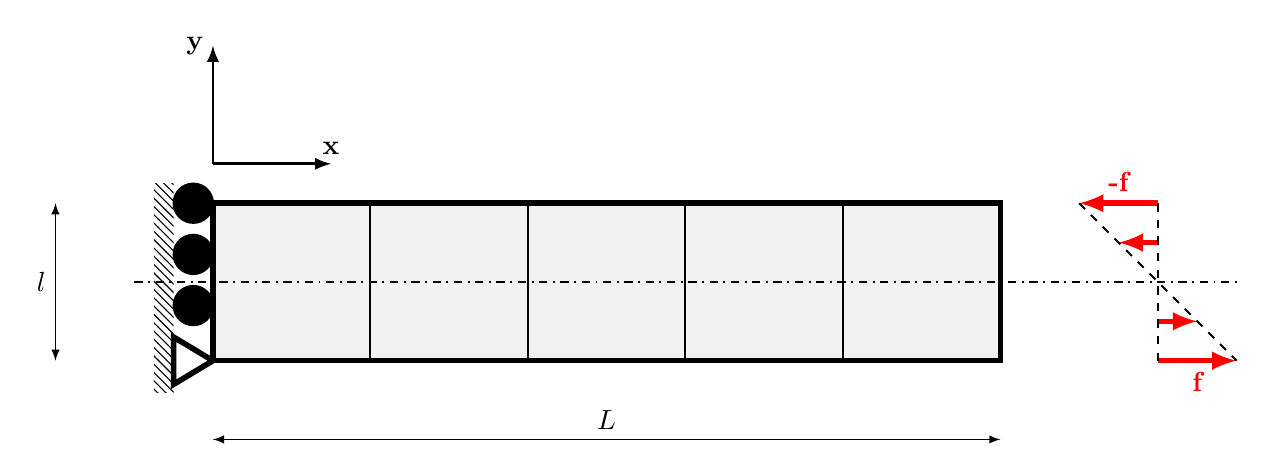
\begin{tikzpicture}[scale = 1.0]
	
	\pgfmathsetmacro{\L}{10}	
 	\pgfmathsetmacro{\l}{2}	
	\pgfmathsetmacro{\dl}{2}
	
	
	\coordinate[](a) at (0,0);
	\coordinate[](b) at (\L,0);	
	\coordinate[](c) at (\L,\l);
	\coordinate[](d) at (0,\l);
	
	\coordinate[](m) at (0,\l/2);
	\coordinate[](mm) at (\L,\l/2);
	
	\coordinate[](t) at (\L+\dl,\l);
	\coordinate[](tt) at (\L+\dl-1,\l);
	\coordinate[](u) at (\L+\dl,0);
	\coordinate[](uu) at (\L+\dl+1,0);
	
	%% Quote
	\coordinate[](ql) at (0, -\dl/2);
	\coordinate[](qll) at (\L, -\dl/2);
	\coordinate[](qh) at (-\dl, 0);
	\coordinate[](qhh) at (-\dl, \l);
		

	% Trave
	\filldraw[fill=gray!10!white, line width=2pt, draw=black] 
	(a) -- (b) -- (c) -- (d) -- cycle;
	
	\begin{scope}[]
	\foreach \x in {1,2,...,4}
	{
	\draw[line width=0.7pt, draw=black] (\x*\dl,  0) -- (\x*\dl,\l);
	}
	\end{scope}	
	
	% Vincoli
	\begin{scope}[]
	\foreach \x in {0,1,...,2}
	{
	\filldraw[fill=black, line width=0.7pt, draw=black] 
	(-0.25,\l-\x*0.65) circle (0.25);
	}
	\end{scope}	
	
	\draw[line width=2pt, draw=black] 
	(a) -- (-0.5,0.3) -- (-0.5,-0.3) -- cycle;
	
	 %% Load
	\begin{scope}[->, ultra thick]
	\draw[->,line width=2.0pt,red] (t) -- (tt) node[red,midway,above]
	{$\textbf{-f}$};
	\draw[->,line width=2.0pt,red] (u) -- (uu) node[red,midway,below]
	{$\textbf{f}$};
	\draw[->,line width=2.0pt,red] (\L+\dl,3*\dl/4) -- (\L+\dl-0.5,3*\dl/4);
	\draw[->,line width=2.0pt,red] (\L+\dl,\dl/4) -- (\L+\dl+0.5,\dl/4);
	\end{scope}	
	\draw[line width=0.7pt, black, dashed] (t) -- (u) ;
	\draw[line width=0.7pt, black, dashed] (tt) -- (uu) ;	
	
	\draw[line width=0.7pt, black, dashdotted] (-1,1) -- (13,1) ;
	%% Quote
	\draw [<->,color=black] (ql) -- (qll) node[black,midway,above] {$L$};
	\draw [<->,color=black] (qh) -- (qhh) node[black,midway,left] {$l$};
	
	% Tratteggio
	\fill[pattern=north west lines, pattern color=black] 
	(-0.75,-0.4) rectangle (-0.5,\l+0.25);
	
	 %% Axis
	\begin{scope}[->, thick]
	\draw[->,line width=1.0pt,black] (0,\l+0.5) -- (0,\l+\dl);
	\draw[->,line width=1.0pt,black] (0,\l+0.5) -- (\l-0.5,\l+0.5);
	\end{scope}	
	\node[black,left] at (0,\l+\dl) {$\textbf{y}$};
	\node[black,above] at (\l-0.5,\l+0.5) {$\textbf{x}$};	
		
\end{tikzpicture}
%\end{center}
%\caption{Beam Cantilever}
%\end{figure}
%
%\end{document}
\caption{Beam cantilever geometry \label{fig:beam_geometry}}
\end{center}
\end{figure}
%
The exact solution is:
\begin{equation}
\begin{split}
&u(x,y) = \frac{2 f}{E l} (1-\nu^{2}) x \left( \frac{l}{2} - y \right)\: , \\
&v(x,y) = \frac{f}{E l} \left[ x^{2} + \frac{\nu}{1-\nu}\left(y^{2}-l y 
\right) \right] \: .
\end{split}
\end{equation}
We use to model the beam two types of mesh: regular anf trapezoidal as in the previously example (see figures \ref{fig:square_regular} and \ref{fig:square_irregular}).
%
\begin{figure}[!h]
\begin{center}
\subfigure[Deformation \label{fig:deformation_beam}]{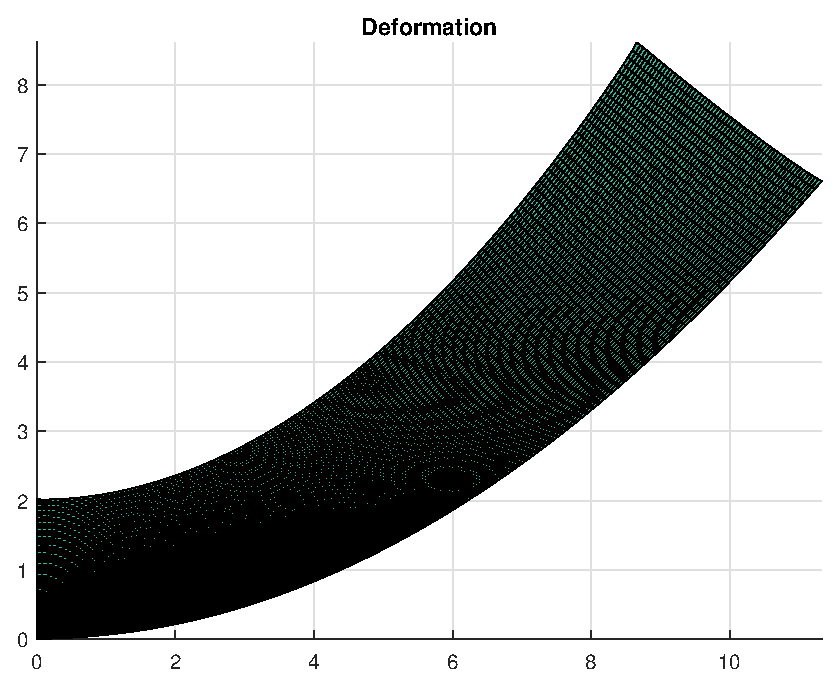
\includegraphics[scale=0.42]{figure/deformata-crop.eps}}\\
\subfigure[Strain $\bm{b}_{xx}$ \label{fig:strain_xx_beam}]{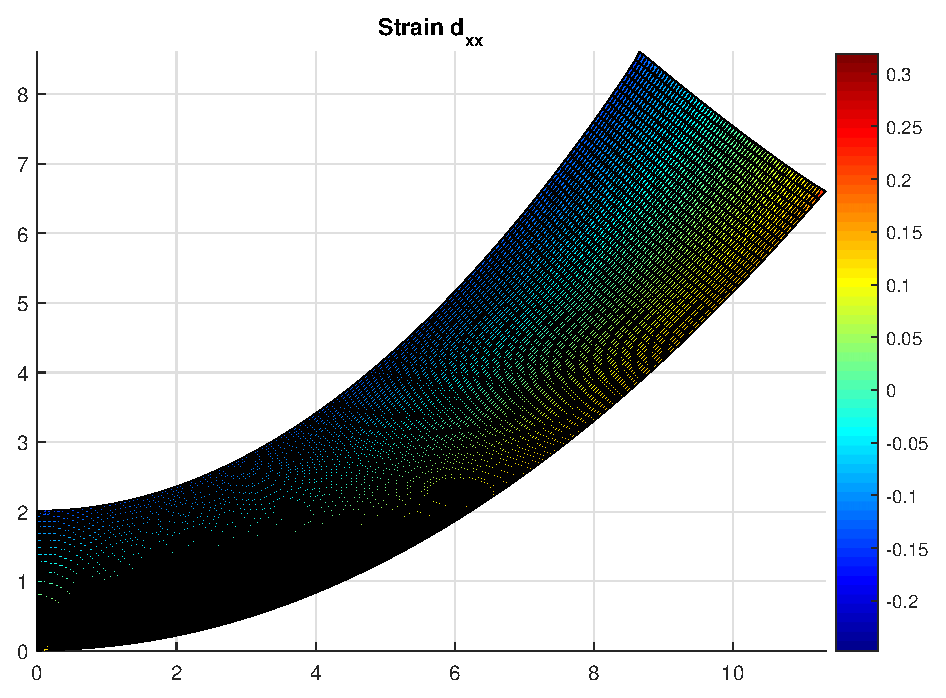
\includegraphics[scale=0.42]{figure/strain_xx-crop.eps}}
\hspace{0.3cm}
\subfigure[Strain $\bm{b}_{yy}$ \label{fig:strain_yy_beam}]{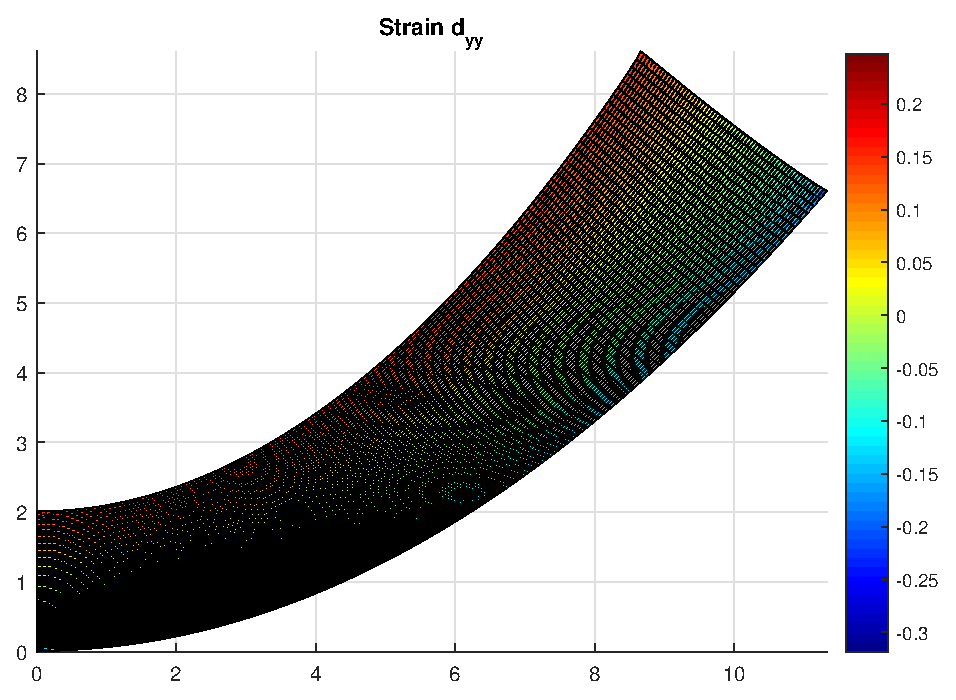
\includegraphics[scale=0.42]{figure/strain_yy-crop.eps}}
\caption{Beam cantilever solution using $8192$ elements of two bubble functions and $\alpha/ \mu=3$}
\end{center}
\end{figure}
%
\begin{figure}[h!]
\begin{center}
\subfigure[Type 1 \label{fig:beam_reg_1B_type1}]
{%\documentclass{article}
%
%\usepackage{graphicx}
%\usepackage{xcolor}
%\usepackage{colortbl}
%\usepackage{fp}
%\usepackage{tikz, pgfplots}
%\usetikzlibrary{calc}
%\usetikzlibrary{patterns}
%\usetikzlibrary{intersections}
%\usetikzlibrary{arrows}
%\tikzset{>=latex}
%
%% Color definition
%\definecolor{green2}{RGB}{154, 205, 50}
%\definecolor{green3}{RGB}{141, 182, 0}
%\definecolor{blue2}{RGB}{0, 102, 255}
%\definecolor{lightgreen}{RGB}{178,255,102}
%
%
%\begin{document}
%\begin{figure}[!h]
%\begin{center}
\begin{tikzpicture}
 \begin{loglogaxis}[width=0.45\textwidth, height=0.45\textwidth,
  legend style={anchor=south, at={(0.5, 1.07)}, draw=none, font=\scriptsize},
  grid=major,
  legend columns=3, transpose legend,
  xlabel={Number of Elements},
  ylabel={$\left(\parallel u_{h}-u \parallel_{L^{2}}\right)/ \parallel u \parallel_{L^{2}}$},
  xmin=1, xmax=1e4,
  ymin=1e-3, ymax=1e0,
  ytick={1e-3, 1e-2, 1e-1, 1},
  yticklabels={$10^{-3}$, $10^{-2}$, $10^{-1}$, $10^{0}$},
  xtick={1e0, 1e1, 1e2, 1e3, 1e4},
  xticklabels={$10^{0}$, $10^{1}$, $10^{2}$, $10^{3}$, $10^{4}$},
 ]
 % Reference
 %\addplot[black, ultra thick] coordinates{
 %(50, 1.8248e-5)
 %(15000, 1.8248e-5)
 %}; 
 %\addlegendentry{Reference} 
 %
 \addplot[red, mark=+, thick, mark options={solid}]
 table [x index={0}, y index={1}]
 {beam_example/regular/bolla1/error_beam_u_l2_type_1_1mu.txt};
 \addlegendentry{$\alpha / \mu=1$}
 %
 \addplot[blue, mark=x, thick, mark options={solid}]
 table [x index={0}, y index={1}]
 {beam_example/regular/bolla1/error_beam_u_l2_type_1_2mu.txt};
 \addlegendentry{$\alpha / \mu=2$}
 %
 \addplot[green3, mark=o, thick, mark options={solid}]
 table [x index={0}, y index={1}]
 {beam_example/regular/bolla1/error_beam_u_l2_type_1_3mu.txt};
 \addlegendentry{$\alpha / \mu=3$}
 %
 %\addplot[red, mark=+, very thick]
 %table [x index={0}, y index={1}]
 %{};
 %\addlegendentry{}
 %
 %\addplot[blue, mark=x, very thick]
 %table [x index={0}, y index={1}]
 %{};
 %\addlegendentry{}
 %
 %\addplot[green3, mark=x, very thick]
 %table [x index={0}, y index={1}]
 %{};
 %\addlegendentry{}
 % 
 \end{loglogaxis}
\end{tikzpicture}
%\end{center}
%\caption{The relative error versus the number of elements measured relative 
%to the $L^{2}$}
%\end{figure}
%
%\end{document}
}
\subfigure[Type 2 \label{fig:beam_reg_1B_type2}]
{%\documentclass{article}
%
%\usepackage{graphicx}
%\usepackage{xcolor}
%\usepackage{colortbl}
%\usepackage{fp}
%\usepackage{tikz, pgfplots}
%\usetikzlibrary{calc}
%\usetikzlibrary{patterns}
%\usetikzlibrary{intersections}
%\usetikzlibrary{arrows}
%\tikzset{>=latex}
%
%% Color definition
%\definecolor{green2}{RGB}{154, 205, 50}
%\definecolor{green3}{RGB}{141, 182, 0}
%\definecolor{blue2}{RGB}{0, 102, 255}
%\definecolor{lightgreen}{RGB}{178,255,102}
%
%
%\begin{document}
%\begin{figure}[!h]
%\begin{center}
\begin{tikzpicture}
 %transpose legend
 \begin{loglogaxis}[width=0.45\textwidth, height=0.45\textwidth,
  legend style={anchor=south, at={(0.5, 1.07)}, draw=none, font=\scriptsize},
  grid=major,
  legend columns=3,
  xlabel={\large Number of Elements},
  ylabel={\Large $\frac{\parallel u_{h}-u \parallel_{L^{2}}}{\parallel u \parallel_{L^{2}}}$},
  xmin=1, xmax=1e4,
  ymin=1e-3, ymax=1e0,
  ytick={1e-3, 1e-2, 1e-1, 1},
  yticklabels={$10^{-3}$, $10^{-2}$, $10^{-1}$, $10^{0}$},
  xtick={1e0, 1e1, 1e2, 1e3, 1e4},
  xticklabels={$10^{0}$, $10^{1}$, $10^{2}$, $10^{3}$, $10^{4}$},
 ]
 % Reference
 %\addplot[black, ultra thick] coordinates{
 %(50, 1.8248e-5)
 %(15000, 1.8248e-5)
 %}; 
 %\addlegendentry{Reference} 
 %
 \addplot[red, mark=+, thick, mark options={solid}]
 table [x index={0}, y index={1}]
 {beam_example/regular/bolla1/error_beam_u_l2_type_2_1mu.txt};
 \addlegendentry{$\alpha / \mu=1$}
 %
 \addplot[blue, mark=x, thick, mark options={solid}]
 table [x index={0}, y index={1}]
 {beam_example/regular/bolla1/error_beam_u_l2_type_2_2mu.txt};
 \addlegendentry{$\alpha / \mu=2$}
 %
 \addplot[green3, mark=o, thick, mark options={solid}]
 table [x index={0}, y index={1}]
 {beam_example/regular/bolla1/error_beam_u_l2_type_2_3mu.txt};
 \addlegendentry{$\alpha / \mu=3$}
 %
 %\addplot[red, mark=+, very thick]
 %table [x index={0}, y index={1}]
 %{};
 %\addlegendentry{}
 %
 %\addplot[blue, mark=x, very thick]
 %table [x index={0}, y index={1}]
 %{};
 %\addlegendentry{}
 %
 %\addplot[green3, mark=x, very thick]
 %table [x index={0}, y index={1}]
 %{};
 %\addlegendentry{}
 % 
 \end{loglogaxis}
\end{tikzpicture}
%\end{center}
%\caption{The relative error versus the number of elements measured relative 
%to the $L^{2}$}
%\end{figure}
%
%\end{document}}
\caption{Beam Cantilever: the relative error vs. the number of elements measured relative to the $L^{2}$ norm (regular mesh)}
\end{center}
\end{figure}
%
\begin{figure}[h!]
\begin{center}
\subfigure[Case two bubble function \label{fig:beam_reg_2B}]
{%\documentclass{article}
%
%\usepackage{graphicx}
%\usepackage{xcolor}
%\usepackage{colortbl}
%\usepackage{fp}
%\usepackage{tikz, pgfplots}
%\usetikzlibrary{calc}
%\usetikzlibrary{patterns}
%\usetikzlibrary{intersections}
%\usetikzlibrary{arrows}
%\tikzset{>=latex}
%
%% Color definition
%\definecolor{green2}{RGB}{154, 205, 50}
%\definecolor{green3}{RGB}{141, 182, 0}
%\definecolor{blue2}{RGB}{0, 102, 255}
%\definecolor{lightgreen}{RGB}{178,255,102}
%
%
%\begin{document}
%\begin{figure}[!h]
%\begin{center}
\begin{tikzpicture}
 %transpose legend
 \begin{loglogaxis}[width=0.45\textwidth, height=0.45\textwidth,
  legend style={anchor=south, at={(0.5, 1.07)}, draw=none, font=\scriptsize},
  grid=major,
  legend columns=3,
  xlabel={\large Number of Elements},
  ylabel={\Large $\frac{\parallel u_{h}-u \parallel_{L^{2}}}{\parallel u \parallel_{L^{2}}}$},
  xmin=1, xmax=1e4,
  ymin=1e-3, ymax=1e0,
  ytick={1e-3, 1e-2, 1e-1, 1},
  yticklabels={$10^{-3}$, $10^{-2}$, $10^{-1}$, $10^{0}$},
  xtick={1e0, 1e1, 1e2, 1e3, 1e4},
  xticklabels={$10^{0}$, $10^{1}$, $10^{2}$, $10^{3}$, $10^{4}$},
 ]
 % Reference
 %\addplot[black, ultra thick] coordinates{
 %(50, 1.8248e-5)
 %(15000, 1.8248e-5)
 %}; 
 %\addlegendentry{Reference} 
 %
 \addplot[red, mark=+, thick, mark options={solid}]
 table [x index={0}, y index={1}]
 {beam_example/regular/bolla2/error_beam_u_l2_1mu.txt};
 \addlegendentry{$\alpha / \mu=1$}
 %
 \addplot[blue, mark=x, thick, mark options={solid}]
 table [x index={0}, y index={1}]
 {beam_example/regular/bolla2/error_beam_u_l2_2mu.txt};
 \addlegendentry{$\alpha / \mu=2$}
 %
 \addplot[green3, mark=o, thick, mark options={solid}]
 table [x index={0}, y index={1}]
 {beam_example/regular/bolla2/error_beam_u_l2_3mu.txt};
 \addlegendentry{$\alpha / \mu=3$}
 %
 %\addplot[red, mark=+, very thick]
 %table [x index={0}, y index={1}]
 %{};
 %\addlegendentry{}
 %
 %\addplot[blue, mark=x, very thick]
 %table [x index={0}, y index={1}]
 %{};
 %\addlegendentry{}
 %
 %\addplot[green3, mark=x, very thick]
 %table [x index={0}, y index={1}]
 %{};
 %\addlegendentry{}
 % 
 \end{loglogaxis}
\end{tikzpicture}
%\end{center}
%\caption{The relative error versus the number of elements measured relative 
%to the $L^{2}$}
%\end{figure}
%
%\end{document}}
\subfigure[Case two bubble function of which one mixed \label{fig:beam_reg_2B_mixed}]
{%\documentclass{article}
%
%\usepackage{graphicx}
%\usepackage{xcolor}
%\usepackage{colortbl}
%\usepackage{fp}
%\usepackage{tikz, pgfplots}
%\usetikzlibrary{calc}
%\usetikzlibrary{patterns}
%\usetikzlibrary{intersections}
%\usetikzlibrary{arrows}
%\tikzset{>=latex}
%
%% Color definition
%\definecolor{green2}{RGB}{154, 205, 50}
%\definecolor{green3}{RGB}{141, 182, 0}
%\definecolor{blue2}{RGB}{0, 102, 255}
%\definecolor{lightgreen}{RGB}{178,255,102}
%
%
%\begin{document}
%\begin{figure}[!h]
%\begin{center}
\begin{tikzpicture}
 %transpose legend
 \begin{loglogaxis}[width=0.45\textwidth, height=0.45\textwidth,
  legend style={anchor=south, at={(0.5, 1.07)}, draw=none, font=\scriptsize},
  grid=major,
  legend columns=3,
  xlabel={Number of Elements},
  ylabel={$\frac{\parallel u_{h}-u \parallel_{L^{2}}}{\parallel u \parallel_{L^{2}}}$},
  xmin=1, xmax=1e4,
  ymin=1e-3, ymax=1e0,
  ytick={1e-3, 1e-2, 1e-1, 1},
  yticklabels={$10^{-3}$, $10^{-2}$, $10^{-1}$, $10^{0}$},
  xtick={1e0, 1e1, 1e2, 1e3, 1e4},
  xticklabels={$10^{0}$, $10^{1}$, $10^{2}$, $10^{3}$, $10^{4}$},
 ]
 % Reference
 %\addplot[black, ultra thick] coordinates{
 %(50, 1.8248e-5)
 %(15000, 1.8248e-5)
 %}; 
 %\addlegendentry{Reference} 
 %
 \addplot[red, mark=+, thick, mark options={solid}]
 table [x index={0}, y index={1}]
 {beam_example/regular/bolla2_mixed/error_beam_u_l2_1mu.txt};
 \addlegendentry{$\alpha / \mu=1$}
 %
 \addplot[blue, mark=x, thick, mark options={solid}]
 table [x index={0}, y index={1}]
 {beam_example/regular/bolla2_mixed/error_beam_u_l2_2mu.txt};
 \addlegendentry{$\alpha / \mu=2$}
 %
 \addplot[green3, mark=o, thick, mark options={solid}]
 table [x index={0}, y index={1}]
 {beam_example/regular/bolla2_mixed/error_beam_u_l2_3mu.txt};
 \addlegendentry{$\alpha / \mu=3$}
 %
 %\addplot[red, mark=+, very thick]
 %table [x index={0}, y index={1}]
 %{};
 %\addlegendentry{}
 %
 %\addplot[blue, mark=x, very thick]
 %table [x index={0}, y index={1}]
 %{};
 %\addlegendentry{}
 %
 %\addplot[green3, mark=x, very thick]
 %table [x index={0}, y index={1}]
 %{};
 %\addlegendentry{}
 % 
 \end{loglogaxis}
\end{tikzpicture}
%\end{center}
%\caption{The relative error versus the number of elements measured relative 
%to the $L^{2}$}
%\end{figure}
%
%\end{document}
}
\caption{Beam Cantilever: the relative error vs. the number of elements measured relative to the $L^{2}$ norm (regular mesh)} 
\end{center}
\end{figure}
we shown in figures \ref{fig:beam_trap_1B_type1}, \ref{fig:beam_trap_1B_type2}, \ref{fig:beam_trap_2B} and \ref{fig:beam_trap_2B_mixed} the $L^{2}$-norm error for different types of bubble functions used in the case of $\alpha/mu:={1,2,3}$, while in figures \ref{fig:beam_trap_1B_type1}, \ref{fig:beam_trap_1B_type2}, \ref{fig:beam_trap_2B} and \ref{fig:beam_trap_2B_mixed} the same plots using trapezoidal meshes.
%% Trapezoidal mesh
\begin{figure}[h!]
\begin{center}
\subfigure[Type 1 \label{fig:beam_trap_1B_type1}]
{%\documentclass{article}
%
%\usepackage{graphicx}
%\usepackage{xcolor}
%\usepackage{colortbl}
%\usepackage{fp}
%\usepackage{tikz, pgfplots}
%\usetikzlibrary{calc}
%\usetikzlibrary{patterns}
%\usetikzlibrary{intersections}
%\usetikzlibrary{arrows}
%\tikzset{>=latex}
%
%% Color definition
%\definecolor{green2}{RGB}{154, 205, 50}
%\definecolor{green3}{RGB}{141, 182, 0}
%\definecolor{blue2}{RGB}{0, 102, 255}
%\definecolor{lightgreen}{RGB}{178,255,102}
%
%
%\begin{document}
%\begin{figure}[!h]
%\begin{center}
\begin{tikzpicture}
 %transpose legend
 \begin{loglogaxis}[width=0.45\textwidth, height=0.45\textwidth,
  legend style={anchor=south, at={(0.5, 1.07)}, draw=none, font=\scriptsize},
  grid=major,
  legend columns=3,
  xlabel={\large Number of Elements},
  ylabel={\Large $\frac{\parallel u_{h}-u \parallel_{L^{2}}}{\parallel u \parallel_{L^{2}}}$},
  xmin=1, xmax=1e4,
  ymin=1e-3, ymax=1e0,
  ytick={1e-3, 1e-2, 1e-1, 1},
  yticklabels={$10^{-3}$, $10^{-2}$, $10^{-1}$, $10^{0}$},
  xtick={1e0, 1e1, 1e2, 1e3, 1e4},
  xticklabels={$10^{0}$, $10^{1}$, $10^{2}$, $10^{3}$, $10^{4}$},
 ]
 % Reference
 %\addplot[black, ultra thick] coordinates{
 %(50, 1.8248e-5)
 %(15000, 1.8248e-5)
 %}; 
 %\addlegendentry{Reference} 
 %
 \addplot[red, mark=+, thick, mark options={solid}]
 table [x index={0}, y index={1}]
 {beam_example/trapezoidal/bolla1/error_beam_u_l2_type_1_dist_1mu.txt};
 \addlegendentry{$\alpha / \mu=1$}
 %
 \addplot[blue, mark=x, thick, mark options={solid}]
 table [x index={0}, y index={1}]
 {beam_example/trapezoidal/bolla1/error_beam_u_l2_type_1_dist_2mu.txt};
 \addlegendentry{$\alpha / \mu=2$}
 %
 \addplot[green3, mark=o, thick, mark options={solid}]
 table [x index={0}, y index={1}]
 {beam_example/trapezoidal/bolla1/error_beam_u_l2_type_1_dist_3mu.txt};
 \addlegendentry{$\alpha / \mu=3$}
 %
 %\addplot[red, mark=+, very thick]
 %table [x index={0}, y index={1}]
 %{};
 %\addlegendentry{}
 %
 %\addplot[blue, mark=x, very thick]
 %table [x index={0}, y index={1}]
 %{};
 %\addlegendentry{}
 %
 %\addplot[green3, mark=x, very thick]
 %table [x index={0}, y index={1}]
 %{};
 %\addlegendentry{}
 % 
 \end{loglogaxis}
\end{tikzpicture}
%\end{center}
%\caption{The relative $L^{2}$ error vs. the number of elements (mesh trapezoidal)}
%\end{figure}
%
%\end{document}
}
\subfigure[Type 2 \label{fig:beam_trap_1B_type2}]
{%\documentclass{article}
%
%\usepackage{graphicx}
%\usepackage{xcolor}
%\usepackage{colortbl}
%\usepackage{fp}
%\usepackage{tikz, pgfplots}
%\usetikzlibrary{calc}
%\usetikzlibrary{patterns}
%\usetikzlibrary{intersections}
%\usetikzlibrary{arrows}
%\tikzset{>=latex}
%
%% Color definition
%\definecolor{green2}{RGB}{154, 205, 50}
%\definecolor{green3}{RGB}{141, 182, 0}
%\definecolor{blue2}{RGB}{0, 102, 255}
%\definecolor{lightgreen}{RGB}{178,255,102}
%
%
%\begin{document}
%\begin{figure}[!h]
%\begin{center}
\begin{tikzpicture}
 %transpose legend
 \begin{loglogaxis}[width=0.45\textwidth, height=0.45\textwidth,
  legend style={anchor=south, at={(0.5, 1.07)}, draw=none, font=\scriptsize},
  grid=major,
  legend columns=3,
  xlabel={\large Number of Elements},
  ylabel={\Large $\frac{\parallel u_{h}-u \parallel_{L^{2}}}{\parallel u \parallel_{L^{2}}}$},
  xmin=1, xmax=1e4,
  ymin=1e-3, ymax=1e0,
  ytick={1e-3, 1e-2, 1e-1, 1},
  yticklabels={$10^{-3}$, $10^{-2}$, $10^{-1}$, $10^{0}$},
  xtick={1e0, 1e1, 1e2, 1e3, 1e4},
  xticklabels={$10^{0}$, $10^{1}$, $10^{2}$, $10^{3}$, $10^{4}$},
 ]
 % Reference
 %\addplot[black, ultra thick] coordinates{
 %(50, 1.8248e-5)
 %(15000, 1.8248e-5)
 %}; 
 %\addlegendentry{Reference} 
 %
 \addplot[red, mark=+, thick, mark options={solid}]
 table [x index={0}, y index={1}]
 {beam_example/trapezoidal/bolla1/error_beam_u_l2_type_2_dist_1mu.txt};
 \addlegendentry{$\alpha / \mu=1$}
 %
 \addplot[blue, mark=x, thick, mark options={solid}]
 table [x index={0}, y index={1}]
 {beam_example/trapezoidal/bolla1/error_beam_u_l2_type_2_dist_2mu.txt};
 \addlegendentry{$\alpha / \mu=2$}
 %
 \addplot[green3, mark=o, thick, mark options={solid}]
 table [x index={0}, y index={1}]
 {beam_example/trapezoidal/bolla1/error_beam_u_l2_type_2_dist_3mu.txt};
 \addlegendentry{$\alpha / \mu=3$}
 %
 %\addplot[red, mark=+, very thick]
 %table [x index={0}, y index={1}]
 %{};
 %\addlegendentry{}
 %
 %\addplot[blue, mark=x, very thick]
 %table [x index={0}, y index={1}]
 %{};
 %\addlegendentry{}
 %
 %\addplot[green3, mark=x, very thick]
 %table [x index={0}, y index={1}]
 %{};
 %\addlegendentry{}
 % 
 \end{loglogaxis}
\end{tikzpicture}
%\end{center}
%\caption{The relative $L^{2}$ error vs. the number of elements (mesh trapezoidal)}
%\end{figure}
%
%\end{document}
}
\caption{Beam Cantilever: the relative error vs. the number of elements measured relative to the $L^{2}$ norm (trapezoidal mesh)}
\end{center}
\end{figure}
%
\begin{figure}[h!]
\begin{center}
\subfigure[Case two bubble function \label{fig:beam_trap_2B}]
{%\documentclass{article}
%
%\usepackage{graphicx}
%\usepackage{xcolor}
%\usepackage{colortbl}
%\usepackage{fp}
%\usepackage{tikz, pgfplots}
%\usetikzlibrary{calc}
%\usetikzlibrary{patterns}
%\usetikzlibrary{intersections}
%\usetikzlibrary{arrows}
%\tikzset{>=latex}
%
%% Color definition
%\definecolor{green2}{RGB}{154, 205, 50}
%\definecolor{green3}{RGB}{141, 182, 0}
%\definecolor{blue2}{RGB}{0, 102, 255}
%\definecolor{lightgreen}{RGB}{178,255,102}
%
%
%\begin{document}
%\begin{figure}[!h]
%\begin{center}
\begin{tikzpicture}
 \begin{loglogaxis}[width=0.45\textwidth, height=0.45\textwidth,
  legend style={anchor=south, at={(0.5, 1.07)}, draw=none, font=\scriptsize},
  grid=major,
  legend columns=3,transpose legend,
  xlabel={Number of Elements},
  ylabel={$\left(\parallel u_{h}-u \parallel_{L^{2}}\right)/ \parallel u \parallel_{L^{2}}$},
  xmin=1, xmax=1e4,
  ymin=1e-3, ymax=1e0,
  ytick={1e-3, 1e-2, 1e-1, 1},
  yticklabels={$10^{-3}$, $10^{-2}$, $10^{-1}$, $10^{0}$},
  xtick={1e0, 1e1, 1e2, 1e3, 1e4},
  xticklabels={$10^{0}$, $10^{1}$, $10^{2}$, $10^{3}$, $10^{4}$},
 ]
 % Reference
 %\addplot[black, ultra thick] coordinates{
 %(50, 1.8248e-5)
 %(15000, 1.8248e-5)
 %}; 
 %\addlegendentry{Reference} 
 %
 \addplot[red, mark=+, thick, mark options={solid}]
 table [x index={0}, y index={1}]
 {beam_example/trapezoidal/bolla2/error_beam_dist_u_l2_1mu.txt};
 \addlegendentry{$\alpha / \mu=1$}
 %
 \addplot[blue, mark=x, thick, mark options={solid}]
 table [x index={0}, y index={1}]
 {beam_example/trapezoidal/bolla2/error_beam_dist_u_l2_2mu.txt};
 \addlegendentry{$\alpha / \mu=2$}
 %
 \addplot[green3, mark=o, thick, mark options={solid}]
 table [x index={0}, y index={1}]
 {beam_example/trapezoidal/bolla2/error_beam_dist_u_l2_3mu.txt};
 \addlegendentry{$\alpha / \mu=3$}
 %
 %\addplot[red, mark=+, very thick]
 %table [x index={0}, y index={1}]
 %{};
 %\addlegendentry{}
 %
 %\addplot[blue, mark=x, very thick]
 %table [x index={0}, y index={1}]
 %{};
 %\addlegendentry{}
 %
 %\addplot[green3, mark=x, very thick]
 %table [x index={0}, y index={1}]
 %{};
 %\addlegendentry
 % 
 \end{loglogaxis}
\end{tikzpicture}
%\end{center}
%\caption{The relative $L^{2}$ error vs. the number of elements (mesh trapezoidal)}
%\end{figure}
%
%\end{document}
}
\subfigure[Case two bubble function of which one mixed 
\label{fig:beam_trap_2B_mixed}]
{%\documentclass{article}
%
%\usepackage{graphicx}
%\usepackage{xcolor}
%\usepackage{colortbl}
%\usepackage{fp}
%\usepackage{tikz, pgfplots}
%\usetikzlibrary{calc}
%\usetikzlibrary{patterns}
%\usetikzlibrary{intersections}
%\usetikzlibrary{arrows}
%\tikzset{>=latex}
%
%% Color definition
%\definecolor{green2}{RGB}{154, 205, 50}
%\definecolor{green3}{RGB}{141, 182, 0}
%\definecolor{blue2}{RGB}{0, 102, 255}
%\definecolor{lightgreen}{RGB}{178,255,102}
%
%
%\begin{document}
%\begin{figure}[!h]
%\begin{center}
\begin{tikzpicture}
 \begin{loglogaxis}[width=0.45\textwidth, height=0.45\textwidth,
  legend style={anchor=south, at={(0.5, 1.07)}, draw=none, font=\scriptsize},
  grid=major,
  legend columns=3, transpose legend,
  xlabel={Number of Elements},
  ylabel={$\left( \parallel u_{h}- u \parallel_{L^{2}}\right)/ \parallel u \parallel_{L^{2}}$},
  xmin=1, xmax=1e4,
  ymin=1e-3, ymax=1e0,
  ytick={1e-3, 1e-2, 1e-1, 1},
  yticklabels={$10^{-3}$, $10^{-2}$, $10^{-1}$, $10^{0}$},
  xtick={1e0, 1e1, 1e2, 1e3, 1e4},
  xticklabels={$10^{0}$, $10^{1}$, $10^{2}$, $10^{3}$, $10^{4}$},
 ]
 % Reference
 %\addplot[black, ultra thick] coordinates{
 %(50, 1.8248e-5)
 %(15000, 1.8248e-5)
 %}; 
 %\addlegendentry{Reference} 
 %
 \addplot[red, mark=+, thick, mark options={solid}]
 table [x index={0}, y index={1}]
 {beam_example/trapezoidal/bolla2_mixed/error_beam_dist_u_l2_1mu.txt};
 \addlegendentry{$\alpha / \mu=1$}
 %
 \addplot[blue, mark=x, thick, mark options={solid}]
 table [x index={0}, y index={1}]
 {beam_example/trapezoidal/bolla2_mixed/error_beam_dist_u_l2_2mu.txt};
 \addlegendentry{$\alpha / \mu=2$}
 %
 \addplot[green3, mark=o, thick, mark options={solid}]
 table [x index={0}, y index={1}]
 {beam_example/trapezoidal/bolla2_mixed/error_beam_dist_u_l2_3mu.txt};
 \addlegendentry{$\alpha / \mu=3$}
 %
 %\addplot[red, mark=+, very thick]
 %table [x index={0}, y index={1}]
 %{};
 %\addlegendentry{}
 %
 %\addplot[blue, mark=x, very thick]
 %table [x index={0}, y index={1}]
 %{};
 %\addlegendentry{}
 %
 %\addplot[green3, mark=x, very thick]
 %table [x index={0}, y index={1}]
 %{};
 %\addlegendentry{}
 % 
 \end{loglogaxis}
\end{tikzpicture}
%\end{center}
%\caption{The relative $L^{2}$ error vs. the number of elements (mesh trapezoidal)}
%\end{figure}
%
%\end{document}
}
\caption{Beam Cantilever: the relative error vs. the number of elements measured relative to the $L^{2}$ norm (trapezoidal mesh)}
\end{center}
\end{figure}
In the all cases the elements distorted have a good behaviour respect to the regular mesh.  

\subsection{Cook's membrane}
The final example is the Cook's membrane. That is a typical benchmark and consist of a beam with vertex: $(0,0)$, $(48,44)$, $(48,60)$ and $(0,44)$.
The left vertical edge is clamped and the right vertical edge subjected to the vertical distributed forces with resultant $F=100$ as it shown in figure \ref{fig:cook}.
%
\begin{figure}[h!]
\begin{center}
%\documentclass{article}
%
%\usepackage{tikz}
%\usepackage{tikz-3dplot}
%\usetikzlibrary{calc}
%\usetikzlibrary{patterns}
%\usetikzlibrary{intersections}
%\usetikzlibrary{arrows}
%\tikzset{>=latex}
%
%\begin{document}
%
%\begin{figure}[!h]
%\begin{center}
\footnotesize
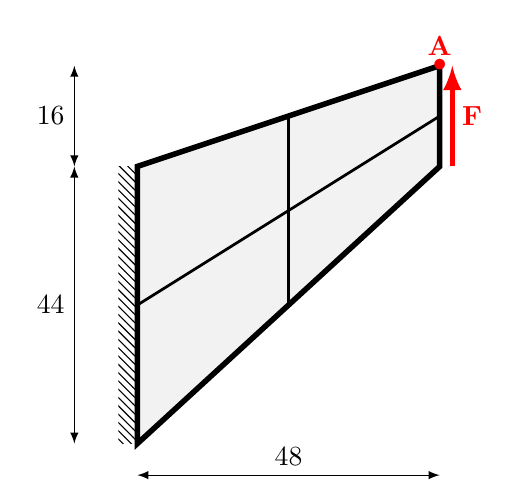
\begin{tikzpicture}[scale = 0.08]
	\coordinate[](a) at (0,0);
	\coordinate[](b) at (48,44);	
	\coordinate[](c) at (48,60);
	\coordinate[](d) at (0,44);
	
	\coordinate[](Mu) at (50,44);
	\coordinate[](Muu) at (50,60);
	\coordinate[](Ml) at (50,52);
	
	\coordinate[](aa) at (0, 22);	
	\coordinate[](bb) at (48,52);
	\coordinate[](cc) at (24,22);
	\coordinate[](dd) at (24,52);
	
	\coordinate[](Ql) at (0,-5);	
	\coordinate[](Qll) at (48,-5);
	\coordinate[](Qh) at (-10,0);	
	\coordinate[](Qhh) at (-10,44);
	\coordinate[](Qhhh) at (-10,60);	
	
	% Trave
	\filldraw[fill=gray!10!white, line width=2pt, draw=black] (a) -- (b) -- (c) -- (d) -- cycle;
	\draw[line width=1pt, black] (aa) -- (bb);
	\draw[line width=1pt, black] (cc) -- (dd);
	
	% Tratteggio
	\fill[pattern=north west lines, pattern color=black] (d) rectangle (-3,0);
	
	 %% Load
	\begin{scope}[->, ultra thick]
	\draw[->,line width=2.0pt,red] (Mu) -- (Muu);
	\end{scope}	
	\node[red,right] at (Ml) {$\textbf{F}$};
		
	\fill[red] node at (c) {$\bullet$};	
	\node[red,above] at (c) {$\textbf{A}$};
	
	%% Quote
	\draw [<->,color=black] (Ql) -- (Qll) node[black,midway,above] {$48$};
	\draw [<->,color=black] (Qh) -- (Qhh) node[black,midway,left] {$44$};
	\draw [<->,color=black] (Qhh) -- (Qhhh) node[black,midway,left] {$16$};
			
\end{tikzpicture}
%\end{center}
%\caption{Cook's Membrane}
%\end{figure}
%
%\end{document}
\caption{Cook's Membrane geometry \label{fig:cook}}
\end{center}
\end{figure}
The material properties are taken to be $E = 250$ and $\nu = 0.4999$, so that a nearly incompressible response is obtained.
We report in figures \ref{fig:cook_alpha_1}, \ref{fig:cook_alpha_1mu}, \ref{fig:cook_alpha_2mu} and \ref{fig:cook_alpha_3mu} the vertical displacement of the point $A$ versus the number of element per side for different choosing of the parameter $\alpha=\left\lbrace 1, \mu, 2\mu, 3\mu \right\rbrace$.
% Alpha 1, 1*mu, 2*mu, 3*mu
\begin{figure}[h!]
\begin{center}
\subfigure[$\alpha=1$ \label{fig:cook_alpha_1}]
{%\documentclass{article}
%
%\usepackage{graphicx}
%\usepackage{xcolor}
%\usepackage{colortbl}
%\usepackage{fp}
%\usepackage{tikz, pgfplots}
%\usetikzlibrary{calc}
%\usetikzlibrary{patterns}
%\usetikzlibrary{intersections}
%\usetikzlibrary{arrows}
%\tikzset{>=latex}
%
%% Color definition
%\definecolor{green2}{RGB}{154, 205, 50}
%\definecolor{green3}{RGB}{141, 182, 0}
%\definecolor{blue2}{RGB}{0, 102, 255}
%\definecolor{lightgreen}{RGB}{178,255,102}
%
%
%\begin{document}
%
%\begin{figure}[!h]
%\begin{center}
\begin{tikzpicture}
 %transpose legend
 \begin{axis}[width=0.45\textwidth, height=0.45\textwidth,
  legend style={anchor=south, at={(0.5, 1.07)}, draw=none, font=\scriptsize},
  legend columns=2,
  xlabel={Number of Elements per Side},
  ylabel={Vertical displacement of point A},
  xmin=0, xmax=32,
  ymin=0, ymax=8,
  ytick={0, 1, 2, 3, 4, 5, 6, 7, 8},
  yticklabels={$0$, $1$, $2$, $3$, $4$, $5$, $6$, $7$, $8$},
  xtick={0, 2, 4, 8, 16, 32},
  xticklabels={$0$, $2$, $4$, $8$, $16$, $32$},
 ]
 % Reference
 %\addplot[black, ultra thick] coordinates{
 %(50, 1.8248e-5)
 %(15000, 1.8248e-5)
 %}; 
 %\addlegendentry{Reference} 
 %
 
 \addplot[red, mark=+, thick, dashed, mark options={solid}]
 table [x index={0}, y index={1}]
 {quad_cook_membrane_graph/alpha_3mu/cook_1B_type_1.txt};
 \addlegendentry{1 Bubble type 1}
 %
 \addplot[red, mark=+, thick, mark options={solid}]
 table [x index={0}, y index={1}]
 {quad_cook_membrane_graph/alpha_3mu/cook_1B_type_2.txt};
 \addlegendentry{1 Bubble type 2}
 % 
 \addplot[green3, mark=o, thick, mark options={solid}]
 table [x index={0}, y index={1}]
 {quad_cook_membrane_graph/alpha_3mu/cook_2B.txt};
 \addlegendentry{2 Bubble}
 %
 \addplot[blue, mark=x, thick, mark options={solid}]
 table [x index={0}, y index={1}]
 {quad_cook_membrane_graph/alpha_3mu/cook_2B_mixed.txt};
 \addlegendentry{2 Bubble Mixed}
 %
 %\addplot[blue, mark=x, very thick]
 %table [x index={0}, y index={1}]
 %{};
 %\addlegendentry{}
 %
 %\addplot[green3, mark=x, very thick]
 %table [x index={0}, y index={1}]
 %{};
 %\addlegendentry{}
 % 
 \end{axis}
\end{tikzpicture}
%\end{center}
%\caption{Vertical Displacement of point A vs. the number of element per side ($\alpha / \mu=3$)}
%\end{figure}
%
%\end{document}
}
\subfigure[$\alpha/ \mu=1$ \label{fig:cook_alpha_1mu}]
{%\documentclass{article}
%
%\usepackage{graphicx}
%\usepackage{xcolor}
%\usepackage{colortbl}
%\usepackage{fp}
%\usepackage{tikz, pgfplots}
%\usetikzlibrary{calc}
%\usetikzlibrary{patterns}
%\usetikzlibrary{intersections}
%\usetikzlibrary{arrows}
%\tikzset{>=latex}
%
%% Color definition
%\definecolor{green2}{RGB}{154, 205, 50}
%\definecolor{green3}{RGB}{141, 182, 0}
%\definecolor{blue2}{RGB}{0, 102, 255}
%\definecolor{lightgreen}{RGB}{178,255,102}
%
%
%\begin{document}
%
%\begin{figure}[!h]
%\begin{center}
\begin{tikzpicture}
 %transpose legend
 \begin{axis}[width=0.45\textwidth, height=0.45\textwidth,
  legend style={anchor=south, at={(0.5, 1.07)}, draw=none, font=\scriptsize},
  legend columns=2,
  xlabel={Number of Elements per Side},
  ylabel={Vertical displacement of point A},
  xmin=0, xmax=32,
  ymin=0, ymax=8,
  ytick={0, 1, 2, 3, 4, 5, 6, 7, 8},
  yticklabels={$0$, $1$, $2$, $3$, $4$, $5$, $6$, $7$, $8$},
  xtick={0, 2, 4, 8, 16, 32},
  xticklabels={$0$, $2$, $4$, $8$, $16$, $32$},
 ]
 % Reference
 %\addplot[black, ultra thick] coordinates{
 %(50, 1.8248e-5)
 %(15000, 1.8248e-5)
 %}; 
 %\addlegendentry{Reference} 
 %
 
 \addplot[red, mark=+, thick, dashed, mark options={solid}]
 table [x index={0}, y index={1}]
 {quad_cook_membrane_graph/alpha_3mu/cook_1B_type_1.txt};
 \addlegendentry{1 Bubble type 1}
 %
 \addplot[red, mark=+, thick, mark options={solid}]
 table [x index={0}, y index={1}]
 {quad_cook_membrane_graph/alpha_3mu/cook_1B_type_2.txt};
 \addlegendentry{1 Bubble type 2}
 % 
 \addplot[green3, mark=o, thick, mark options={solid}]
 table [x index={0}, y index={1}]
 {quad_cook_membrane_graph/alpha_3mu/cook_2B.txt};
 \addlegendentry{2 Bubble}
 %
 \addplot[blue, mark=x, thick, mark options={solid}]
 table [x index={0}, y index={1}]
 {quad_cook_membrane_graph/alpha_3mu/cook_2B_mixed.txt};
 \addlegendentry{2 Bubble Mixed}
 %
 %\addplot[blue, mark=x, very thick]
 %table [x index={0}, y index={1}]
 %{};
 %\addlegendentry{}
 %
 %\addplot[green3, mark=x, very thick]
 %table [x index={0}, y index={1}]
 %{};
 %\addlegendentry{}
 % 
 \end{axis}
\end{tikzpicture}
%\end{center}
%\caption{Vertical Displacement of point A vs. the number of element per side ($\alpha / \mu=3$)}
%\end{figure}
%
%\end{document}
}
\subfigure[$\alpha/ \mu=2$ \label{fig:cook_alpha_2mu}]
{%\documentclass{article}
%
%\usepackage{graphicx}
%\usepackage{xcolor}
%\usepackage{colortbl}
%\usepackage{fp}
%\usepackage{tikz, pgfplots}
%\usetikzlibrary{calc}
%\usetikzlibrary{patterns}
%\usetikzlibrary{intersections}
%\usetikzlibrary{arrows}
%\tikzset{>=latex}
%
%% Color definition
%\definecolor{green2}{RGB}{154, 205, 50}
%\definecolor{green3}{RGB}{141, 182, 0}
%\definecolor{blue2}{RGB}{0, 102, 255}
%\definecolor{lightgreen}{RGB}{178,255,102}
%
%
%\begin{document}
%
%\begin{figure}[!h]
%\begin{center}
\begin{tikzpicture}
 %transpose legend
 \begin{axis}[width=0.45\textwidth, height=0.45\textwidth,
  legend style={anchor=south, at={(0.5, 1.07)}, draw=none, font=\scriptsize},
  legend columns=2,
  xlabel={Number of Elements per Side},
  ylabel={Vertical displacement of point A},
  xmin=0, xmax=32,
  ymin=0, ymax=8,
  ytick={0, 1, 2, 3, 4, 5, 6, 7, 8},
  yticklabels={$0$, $1$, $2$, $3$, $4$, $5$, $6$, $7$, $8$},
  xtick={0, 2, 4, 8, 16, 32},
  xticklabels={$0$, $2$, $4$, $8$, $16$, $32$},
 ]
 % Reference
 %\addplot[black, ultra thick] coordinates{
 %(50, 1.8248e-5)
 %(15000, 1.8248e-5)
 %}; 
 %\addlegendentry{Reference} 
 %
 
 \addplot[red, mark=+, thick, dashed, mark options={solid}]
 table [x index={0}, y index={1}]
 {quad_cook_membrane_graph/alpha_3mu/cook_1B_type_1.txt};
 \addlegendentry{1 Bubble type 1}
 %
 \addplot[red, mark=+, thick, mark options={solid}]
 table [x index={0}, y index={1}]
 {quad_cook_membrane_graph/alpha_3mu/cook_1B_type_2.txt};
 \addlegendentry{1 Bubble type 2}
 % 
 \addplot[green3, mark=o, thick, mark options={solid}]
 table [x index={0}, y index={1}]
 {quad_cook_membrane_graph/alpha_3mu/cook_2B.txt};
 \addlegendentry{2 Bubble}
 %
 \addplot[blue, mark=x, thick, mark options={solid}]
 table [x index={0}, y index={1}]
 {quad_cook_membrane_graph/alpha_3mu/cook_2B_mixed.txt};
 \addlegendentry{2 Bubble Mixed}
 %
 %\addplot[blue, mark=x, very thick]
 %table [x index={0}, y index={1}]
 %{};
 %\addlegendentry{}
 %
 %\addplot[green3, mark=x, very thick]
 %table [x index={0}, y index={1}]
 %{};
 %\addlegendentry{}
 % 
 \end{axis}
\end{tikzpicture}
%\end{center}
%\caption{Vertical Displacement of point A vs. the number of element per side ($\alpha / \mu=3$)}
%\end{figure}
%
%\end{document}
}
\subfigure[$\alpha/ \mu=3$ \label{fig:cook_alpha_3mu}]
{%\documentclass{article}
%
%\usepackage{graphicx}
%\usepackage{xcolor}
%\usepackage{colortbl}
%\usepackage{fp}
%\usepackage{tikz, pgfplots}
%\usetikzlibrary{calc}
%\usetikzlibrary{patterns}
%\usetikzlibrary{intersections}
%\usetikzlibrary{arrows}
%\tikzset{>=latex}
%
%% Color definition
%\definecolor{green2}{RGB}{154, 205, 50}
%\definecolor{green3}{RGB}{141, 182, 0}
%\definecolor{blue2}{RGB}{0, 102, 255}
%\definecolor{lightgreen}{RGB}{178,255,102}
%
%
%\begin{document}
%
%\begin{figure}[!h]
%\begin{center}
\begin{tikzpicture}
 %transpose legend
 \begin{axis}[width=0.45\textwidth, height=0.45\textwidth,
  legend style={anchor=south, at={(0.5, 1.07)}, draw=none, font=\scriptsize},
  legend columns=2,
  xlabel={Number of Elements per Side},
  ylabel={Vertical displacement of point A},
  xmin=0, xmax=32,
  ymin=0, ymax=8,
  ytick={0, 1, 2, 3, 4, 5, 6, 7, 8},
  yticklabels={$0$, $1$, $2$, $3$, $4$, $5$, $6$, $7$, $8$},
  xtick={0, 2, 4, 8, 16, 32},
  xticklabels={$0$, $2$, $4$, $8$, $16$, $32$},
 ]
 % Reference
 %\addplot[black, ultra thick] coordinates{
 %(50, 1.8248e-5)
 %(15000, 1.8248e-5)
 %}; 
 %\addlegendentry{Reference} 
 %
 
 \addplot[red, mark=+, thick, dashed, mark options={solid}]
 table [x index={0}, y index={1}]
 {quad_cook_membrane_graph/alpha_3mu/cook_1B_type_1.txt};
 \addlegendentry{1 Bubble type 1}
 %
 \addplot[red, mark=+, thick, mark options={solid}]
 table [x index={0}, y index={1}]
 {quad_cook_membrane_graph/alpha_3mu/cook_1B_type_2.txt};
 \addlegendentry{1 Bubble type 2}
 % 
 \addplot[green3, mark=o, thick, mark options={solid}]
 table [x index={0}, y index={1}]
 {quad_cook_membrane_graph/alpha_3mu/cook_2B.txt};
 \addlegendentry{2 Bubble}
 %
 \addplot[blue, mark=x, thick, mark options={solid}]
 table [x index={0}, y index={1}]
 {quad_cook_membrane_graph/alpha_3mu/cook_2B_mixed.txt};
 \addlegendentry{2 Bubble Mixed}
 %
 %\addplot[blue, mark=x, very thick]
 %table [x index={0}, y index={1}]
 %{};
 %\addlegendentry{}
 %
 %\addplot[green3, mark=x, very thick]
 %table [x index={0}, y index={1}]
 %{};
 %\addlegendentry{}
 % 
 \end{axis}
\end{tikzpicture}
%\end{center}
%\caption{Vertical Displacement of point A vs. the number of element per side ($\alpha / \mu=3$)}
%\end{figure}
%
%\end{document}
}
\caption{Vertical Displacement of point A vs. 
the number of elements per side}
\end{center}
\end{figure}
All elements return different behaviour using different coefficients $\alpha$. In the case of $\alpha=1$, figure \ref{fig:cook_alpha_1}, the obtained results completely not converge to the reference solution.

\section{Conclusions}\label{sec:six}
We present a new family of quadrilaterals mixed finite elements based on a modified Hu-Washizu formulation.
We test the different types of enrichment and confirm the robustness of all elements created.
Uniform convergence are archived in the incompressible regime.
We study the robustness of the elements in the case of trapezoidal meshes.
The extension to the 3D case using hexahedra is straightforward. 

%% The Appendices part is started with the command \appendix;
%% appendix sections are then done as normal sections
%% \appendix

%% \section{}
%% \label{}

%% If you have bibdatabase file and want bibtex to generate the
%% bibitems, please use
%%
%%  \bibliographystyle{elsarticle-harv} 
%%  \bibliography{<your bibdatabase>}

%% else use the following coding to input the bibitems directly in the
%% TeX file.

\begin{thebibliography}{00}
% 1
\bibitem[W.Bai (1997)]{bai} W.Bai. 
``The quadrilateral `Mini' finite element for Stokes problem'',
{\it{Comput. Methods Appl. Mech. Engrg.}}, 143: 41-47, 1997.
% 2
\bibitem[D.Boffi (2006)]{boffi} D.Boffi. ``On the finite element method on quadrilateral meshes", 
{\it{Appl. Num. Mathematics}}, 56: 1271-1282, 2006.
% 3
\bibitem[B.P.Lamichhane (2015)]{lamichhane} B.P.Lamichhane. ``A quadrilateral `mini' finite element for the  Stokes problem using a single bubble function", {\it{Appl. Num. Math.}}, 56: 1271-1282, 2015. 
% 4
\bibitem[J.K.Djoko and B.D.Reddy (2006)]{djoko} J.K.Djoko, B.D.Reddy. ``An extended Hu-Washizu formulation for elasticity", {\it{Comput. Methods Appl. Mech. Engrg.}}, 195: 6330-6346, 2006. 
% 5
\bibitem[B.P.Lamichhane et al. (2013)]{lamichhane_three} B.P.Lamichhane, A.T.McBride, B.D.Reddy. ``A finite element method for three-field formulation of linear elasticity based on biorthogonal systems", 
{\it{Comput. Methods Appl. Mech. Engrg.}}, 258: 109-117, 2013.
% 6
\bibitem[B.P.Lamichhane et al. (2006)]{lamichhane_conv} B.P.Lamichhane, B.D.Reddy, B.I.Wohlmuth. ``Convergence in the incompressible limit of finite element approximation based on Hu-Washizu formulation", 
{\it{Numer. Math.}}, 104: 151-175, 2006.
% 7
\bibitem[D.Boffi and C.Lovadina (1997)]{boffi_lovadina} D.Boffi, C.Lovadina. ``Analisys of new augmented Lagrangian formulation for mixed finite element schemes", 
{\it{Numer. Math.}}, 75: 405-419, 1997.
% 8
\bibitem[B.P.Lamichhane (2009)]{lamichhane_huwashizu} B.P.Lamichhane. ``From the Hu-Washizu formulation to the average nodal strain formulation", 
{\it{Comput. Methods Appl. Mech. Engrg.}}, 198: 3957-3961, 2009.
% 9
\bibitem[D.N.Arnold and R.Winther (2002)]{arnold} D.N.Arnold, R.Winther. ``Mixed finite elements for elasticity", 
{\it{Numer. Math.}}, 92: 401-419, 2002.
% 10
\bibitem[D.Boffi et al. (2013)]{boffi_book} D.Boffi, F.Brezzi, M.Fortin. ``Mixed Finite Element Methods and Applications", 
{\it{Springer Series in Computational Mathematics}}, Vol.44, 2013.
% 11
\bibitem[D.N.Arnold and G.Awanou (2005)]{arnold_quad} D.N.Arnold, G.Awanou. ``Rectangular mixed finite elements for elasticity", 
{\it{Models Methods Appl. Sci.}}, 15: 1417-1429, 2005.
% 12
\bibitem[H.Hu (1955)]{hu} H.Hu. ``On some variational principles in the theory of elasticity and the theory of plasticity", 
{\it{Sci. Sin.}}, 4: 33-54, 1955.
% 13
\bibitem[K.Washizu (1982)]{washizu} K.Washizu. ``Variational Methods in Elasticity and Plasticity, third ed.", 
{\it{Pergamon Press}}, 1982.
% 14
\bibitem[B.M.Fraeijs de Veubeke (1951)]{veubeke} B.M. Fraeijs de Veubeke. ``Diffusion des inconnues hyperstatiques dans les voilures á longeron couplés", {\it{Bull. Serv. Technique de l’Aeronautique Impremérie Marcel Hayez}}, Bruxelles, 1951.
% 15
\bibitem[E.P. Kasper and R.L. Taylor (2000)]{kasper_p1} E.P. Kasper, R.L. Taylor. ``A mixed-enhanced strain method Part I: geometrically linear problems", 
{\it{Comput. Struct.}}, 75: 237-250, 2000.
% 16
\bibitem[E.P. Kasper and R.L. Taylor (2000)]{kasper_p2} E.P. Kasper, R.L. Taylor. ``A mixed-enhanced strain method Part II: geometrically nonlinear problems", 
{\it{Comput. Struct.}}, 75: 251-260, 2000.
% 17
\bibitem[S.C. Brenner (1993)]{brenner} S.C. Brenner. ``A nonconforming mixed multigrid method for the pure displacement problem in planar linear elasticity", 
{\it{SIAM J. Numer. Anal.}}, 30: 116–135, 1993.

\end{thebibliography}
\end{document}

\endinput